\chapter{Real World Applications} \label{chap:realworld}

This chapter presents three applications addressing the \ac{RQ}s, specific objectives, and contributions of this thesis.

The first application is based on \citeonline{dasilva2020Forecasting} entitled ``Forecasting Brazilian and American COVID-19 cases based on \ac{AI} coupled with exogenous climatic variables'' and published in the \textit{Chaos, Solitons \& Fractals} Journal (v.139, June 2020, 110027, \url{https://doi.org/10.1016/j.chaos.2020.110027}). This article mainly explores using signal decomposition methods in time series forecasting.

Next, the second application is based on \citeonline{dasilva2021Novel} entitled ``A novel decomposition-ensemble learning framework for multi-step ahead wind energy forecasting'' and published in \textit{Energy} Journal (v.216, February 2021, 119174, \url{https://doi.org/10.1016/j.energy.2020.119174}). This application aims to combine signal decomposition methods and a stacking-ensemble learning approach. This research is an extension of a sequence of articles that started with \citeonline{moreno2019Very} entitled ``Very short-term wind energy forecasting based on stacking ensemble'' exploring the use of \ac{STACK}, and \citeonline{dasilva2020Wind} entitled ``Wind energy multi-step ahead forecasting based on variational mode decomposition'' using signal decomposition methods to forecast renewable energy time series.

Last, the third application is based on \citeonline{dasilva2022Multistep} entitled ``Multi-step short-term wind speed forecasting based on multi-stage decomposition coupled with stacking-ensemble learning approach'' and published in the \textit{International Journal of Electrical Power \& Energy Systems} Journal (v.143, 108504, December 2022, \url{https://doi.org/10.1016/j.ijepes.2022.108504}). This case aims to apply the multi-stage decomposition strategy coupled with the \ac{STACK} approach. Also, this study was an extension of all applications cited before. Moreover, this forecasting framework was inspired by \citeonline{moreno2020Multistep} entitled ``Multi-step wind speed forecasting based on hybrid multi-stage decomposition model and long short-term memory neural network'' and \citeonline{dasilva2021Multistep} entitled ``Multi-step wind speed forecasting based on multi-stage decomposition approach''. Both studies applied only the multi-stage decomposition strategy, which motivated the author to combine the \ac{STACK} approach to enhance the forecasting framework. Figure \ref{fig:case_studies} summarizes the structure of the applications presented in this chapter.

\begin{figure}[htb!]
    \centering
    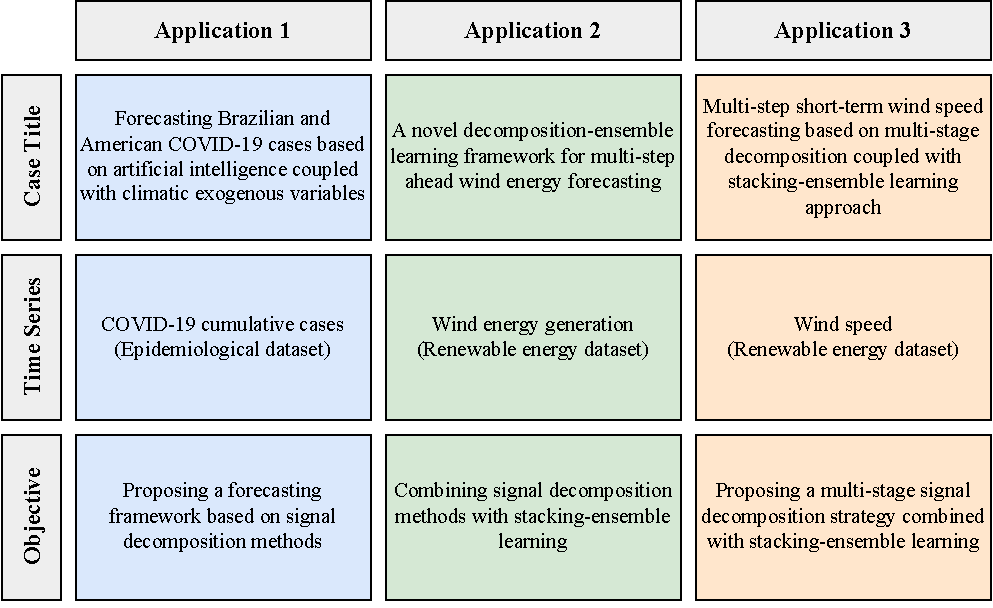
\includegraphics[width=\linewidth]{Media/case_studies.pdf}
    \caption{Applications structure}
    \label{fig:case_studies}
    \source{Author (2023)}
\end{figure}


\newpage
\section{Epidemiological Time Series} \label{sec:epidemio}

This subsection presents a contextualization, contributions, datasets, and methodology adopted for application 1.

%%%%%%%%%%%%%%%%%%%%%%%%%%%%%%%%%%%%%%%%%%%%%%%%%%

\subsection{Contextualization and Contributions}

The \ac{COVID-19} is a viral infectious disease induced by \ac{SARS-CoV2}. According to the \ac{WHO}, most of the population will have mild to moderate respiratory illness and recover without requiring special treatment \cite{worldhealthorganizationwho2020Coronavirus}. However, several studies are being developed, and preliminary results indicated that people with underlying medical problems like cardiovascular disease, diabetes, chronic respiratory disease, obesity, and cancer are more likely to develop serious injuries \cite{bansal2020Cardiovascular,lai2020Severe,hussain2020COVID19,moujaess2020Cancer,abbas2020Mutual,su2020Renal}. Also, the \ac{COVID-19} can cause extensive, and multiple lung injuries \cite{guan2020Clinical}, thus compromising the respiratory system of patients. In this context, the demand for devices that assist in performing breathing-related movements has increased. 

Due to the severe damage caused by \ac{COVID-19}, according to \ac{WHO}, up to June 10th, 2020, more than 7.1 million people were already infected, as well as more than 400 thousand people worldwide have now died with the coronavirus. Indeed, considering the current scenario of the health system worldwide, overcrowding could be observed in some countries like Italy, Spain, and perhaps Brazil. In Brazil, it is believed that an average of 3,388 municipalities could have a significant deficit in hospital beds. Significantly, the debt is projected to occur in Brazilian North and Northeast regions, exceeding health care capacity due to the \ac{COVID-19} \cite{requia2020Risk}. 

In this respect, for forecasting cumulative cases of \ac{COVID-19}, the objective of this study is to explore and compare the predictive capacity of \ac{BRNN}, \ac{CUBIST}, \ac{KNN}, \ac{QRF}, and \ac{SVR} when are used stand-alone, and a hybrid framework composed by \ac{VMD} coupled with previously mentioned models. In this study were used as datasets the number of cumulative cases of \ac{COVID-19} from five Brazilian states (\ac{AM}, \ac{CE}, \ac{PE}, \ac{RJ}, and \ac{SP}), the first state from the north region, the second and third states from the northeast region, and the other two states from the southeast region. Also were considered five  American states (\ac{CA}, \ac{IL}, \ac{MA}, \ac{NJ}, and \ac{NY}). These states were chosen through the most significant number of new cases of \ac{COVID-19} up to April 28th, 2020.  

Forecasting horizons of the time series one, three, and six days ahead of cumulative \ac{COVID-19} cases are adopted to evaluate the forecasting efficiency of the different models. Additionally, previous \ac{COVID-19} cases and exogenous variables such as daily temperature (maximum and minimum) and precipitation are employed as inputs for each evaluated model. The output-of-sample forecasting accuracy of each model is compared by performance metrics such as the \ac{IP}, \ac{sMAPE}, and \ac{RRMSE}. Also, the importance of each input variable is presented for each mentioned country.

Forecasting models are impacted by the small dataset effect and the prediction of cases of \ac{COVID-19}, making a challenging task. The forecasting and preprocessing approaches are chosen because even though nonlinear and \ac{AI} models need large datasets to properly learn the data pattern, the use of exogenous variables (climate variables) and past values of the response variable overcomes this drawback.

\ac{VMD} decomposes a time series into its \ac{IMF}s adaptively and non-recursively, obtaining a set of sub-series with different features from low-frequency to high-frequency. Adopting \ac{VMD} with modes in conjunction with nonlinear machine learning prediction models is a robust framework to approach small datasets in forecasting tasks. In addition, \ac{BRNN} and \ac{SVR} approaches can handle small samples, making them attractive for this study. In consideration of the objectives of this application, the following \ac{RQ}s are defined:

\begin{enumerate}[wide=0pt, leftmargin=3em]
    \item[\textbf{RQ 1.1}] Can signal decomposition approaches enhance the performance of forecasting \ac{COVID-19} cumulative cases time series?
    
    \item[\textbf{RQ 2}] How does the use of exogenous features impact performance improvement when forecasting \ac{COVID-19} cumulative cases time series?
\end{enumerate}

To address the \ac{RQ}s of this application, the contributions can be summarized as follows: 

\begin{enumerate}[label=\alph*)]
    \item The first contribution is related to the proposal of two frameworks, non-decomposed and decomposed models, applied to forecast the new cumulative cases of \ac{COVID-19} in five Brazilian and American states. These evaluated models are expected to be used as the most accurate approaches to perform decision-making to structure the health system, avoid overcrowding in hospitals, and prevent new deaths. 
    
    \item The second contribution, we can highlight the use of a distinct set of \ac{AI} models based on machine learning approaches regarding learning structure, even as the recent effective preprocessing \ac{VMD} to forecasting the Brazilian and American \ac{COVID-19} new cumulative cases. The forecasting models \ac{BRNN}, \ac{CUBIST}, \ac{KNN}, \ac{QRF}, \ac{SVR}, and preprocessing \ac{VMD} method were chosen once they have reached success in several fields of regression and time series forecasting \cite{ribeiro2018Multiobjective,fernandez-delgado2019Extensive,zuo2020Decomposition,zhu2019Hybrid}; 
    
    \item Also, this study evaluates \ac{AI} models in a multi-day-ahead forecasting strategy coupled with exogenous climatic inputs. The range of the forecasting time horizon allows us to verify the effectiveness of the predicting models in different scenarios associated with information such as previous \ac{COVID-19} cumulative cases, temperature, and precipitation, allowing the models to achieve high forecasting accuracy. Finally, their results can help plan actions to improve the health system to contain the \ac{COVID-19} deaths.
\end{enumerate}

%%%%%%%%%%%%%%%%%%%%%%%%%%%%%%%%%%%%%%%%%%%%%%%%%%

\subsection{Dataset Description}

The collected dataset refers to the \ac{COVID-19} cumulative cases that occurred in five states of Brazil and \ac{USA} until April 20th, 2020. For the Brazilian context, the dataset was collected from an API (Application Program Interface) \cite{justen2020COVID19} that retrieves the daily information about \ac{COVID-19} cases from all 27 Brazilian State Health Offices, assembles and makes them publicly available. And for \ac{USA} context, the dataset was collected from ``\ac{COVID-19} Data Repository'' on Github provided by the \ac{CSSE} at Johns Hopkins University \cite{centerforsystemsscienceandengineeringcsse2020Novel}. The cumulative confirmed cases and deaths of each state, and the period from the first and last reports, are illustrated in Table~\ref{tab:reports}. 

% TABLE - Confirmed cases data
\begin{table}[htb!]
\small
\centering
\caption{Summary of COVID-19 cases by country and state}
\label{tab:reports}
\resizebox{\textwidth}{!}{%
\begin{tabular}{ccccccc}
\hline
\textbf{Country} &
  \textbf{State} &
  \textbf{Number of observed days} &
  \textbf{Fist reported} &
  \textbf{Last reported} &
  \textbf{Cumulative cases} &
  \textbf{Cumulative deaths} \\ \hline
\multirow{5}{*}{Brazil} & \ac{AM} & 47 & 13/03/2020 & 28/04/2020 & 4337   & 351   \\
                        & \ac{CE} & 44 & 16/03/2020 & 28/04/2020 & 6985   & 403   \\
                        & \ac{PE} & 48 & 12/03/2020 & 28/04/2020 & 5724   & 508   \\
                        & \ac{RJ} & 55 & 05/03/2020 & 28/04/2020 & 8504   & 738   \\
                        & \ac{SP} & 64 & 25/02/2020 & 28/04/2020 & 24041  & 2049  \\ \hline
\multirow{5}{*}{\ac{USA}}    & \ac{CA} & 94 & 26/01/2020 & 28/04/2020 & 46164  & 1864  \\
                        & \ac{IL} & 96 & 24/01/2020 & 28/04/2020 & 48102  & 2125  \\
                        & \ac{MA} & 87 & 01/02/2020 & 27/04/2020 & 56462  & 3003  \\
                        & \ac{NJ} & 55 & 05/03/2020 & 28/04/2020 & 113856 & 6442  \\
                        & \ac{NY} & 58 & 02/03/2020 & 28/04/2020 & 295106 & 22912 \\ \hline
\end{tabular}
}
\end{table}

The exogenous climatic variables were retrieved from the \ac{INMET} \cite{brazil2020Instituto} for data from Brazil, while the \ac{USA} climate dataset was taken into a count from the daily global historical climatology network that was retrieved from the \ac{NCEI} from the National Oceanic and Atmospheric Administration \cite{u.s.2020National}, by using \texttt{\{rnoaa\}} package \cite{chamberlain2020Rnoaa}. For each state, considering the daily available information, minimum and maximum temperature (\textit{ºC}) and precipitation (\textit{mm}) were selected as exogenous climatic inputs to each forecasting model applied in this study. The measurement period of each state is variable. This is because the record of the first case of the disease may differ from state to state. The summary of the climatic variables used is described in Table \ref{tab:climatic}.  

\begin{scriptsize}
\begin{center}
\begin{longtable}[htb!]{cclcccc}
\caption{Descriptive measures for climatic variables by country and state \label{tab:climatic}}\\
\hline
\textbf{Country} & \textbf{State} & \textbf{Variable} & \textbf{Minimum} & \textbf{Median} & \textbf{Mean} & \textbf{Maximum} \\ \hline \endfirsthead
  \multicolumn{7}{c}%
  {\tablename\ \thetable\ -- \textit{Continued from previous page}} \\ \hline
\textbf{Country} & \textbf{State} & \textbf{Variable} & \textbf{Minimum} & \textbf{Median} & \textbf{Mean} & \textbf{Maximum} \\ \hline \endhead \hline \multicolumn{7}{r}{\textit{Continued on next page}} \\
\endfoot
\hline
\endlastfoot

\multirow{15}{*}{Brazil} & \ac{AM} & Minimum temperature (\textit{ºC}) & 24.76 & 26.20 & 26.36 & 28.28 \\
 &  & Maximum temperature (\textit{ºC}) & 25.29 & 27.05 & 27.24 & 29.55 \\
 &  & Precipitation (\textit{mm}) & 0.00 & 0.11 & 0.33 & 2.40 \\ \cline{2-7}
 & \ac{CE} & Minimum temperature (\textit{ºC}) & 25.14 & 26.62 & 26.60 & 27.90 \\
 &  & Maximum temperature (\textit{ºC}) & 25.91 & 27.73 & 27.68 & 28.99 \\
 &  & Precipitation (\textit{mm}) & 0.00 & 0.12 & 0.25 & 1.31 \\ \cline{2-7}
 & \ac{PE} & Minimum temperature (\textit{ºC}) & 23.36 & 25.18 & 25.05 & 26.74 \\
 &  & Maximum temperature (\textit{ºC}) & 24.27 & 26.30 & 26.10 & 27.96 \\
 &  & Precipitation (\textit{mm}) & 0.00 & 0.14 & 0.23 & 1.33 \\ \cline{2-7}
 & \ac{RJ} & Minimum temperature (\textit{ºC}) & 19.07 & 21.23 & 21.57 & 25.33 \\
 &  & Maximum temperature (\textit{ºC}) & 19.69 & 22.16 & 22.56 & 26.49 \\
 &  & Precipitation (\textit{mm}) & 0.00 & 0.03 & 0.13 & 1.32 \\ \cline{2-7}
 & \ac{SP} & Minimum temperature (\textit{ºC}) & 17.60 & 19.99 & 20.09 & 23.40 \\
 &  & Maximum temperature (\textit{ºC}) & 18.76 & 21.11 & 21.37 & 25.03 \\
 &  & Precipitation (\textit{mm}) & 0.00 & 0.00 & 0.12 & 1.19 \\ \hline
\multirow{15}{*}{\ac{USA}} & {\ac{CA}} & Minimum temperature (\textit{ºC}) & -1.76 & 4.90 & 4.91 & 11.92 \\
 &  & Maximum temperature (\textit{ºC}) & 10.60 & 18.33 & 18.54 & 28.59 \\
 &  & Precipitation (\textit{mm}) & 0.01 & 4.66 & 20.98 & 162.67 \\ \cline{2-7}
 & \ac{IL} & Minimum temperature (\textit{ºC}) & -19.42 & -0.42 & -0.75 & 14.63 \\
 &  & Maximum temperature (\textit{ºC}) & -6.39 & 8.40 & 8.99 & 26.06 \\
 &  & Precipitation (\textit{mm}) & 0.00 & 4.29 & 23.30 & 196.47 \\ \cline{2-7}
 & \ac{MA} & Minimum temperature (\textit{ºC}) & -14.75 & -0.86 & -1.76 & 5.39 \\
 &  & Maximum temperature (\textit{ºC}) & -2.77 & 8.32 & 8.16 & 18.70 \\
 &  & Precipitation (\textit{mm}) & 0.00 & 6.84 & 34.66 & 320.86 \\ \cline{2-7}
 & \ac{NJ} & Minimum temperature (\textit{ºC}) & -11.80 & 1.60 & 0.96 & 7.27 \\
 &  & Maximum temperature (\textit{ºC}) & 0.54 & 10.78 & 11.22 & 22.02 \\
 &  & Precipitation (\textit{mm}) & 0.00 & 5.44 & 31.53 & 274.04 \\ \cline{2-7}
 & \ac{NY} & Minimum temperature (\textit{ºC}) & -20.48 & -2.61 & -3.75 & 4.60 \\
 &  & Maximum temperature (\textit{ºC}) & -7.98 & 5.62 & 6.23 & 17.88 \\
 &  & Precipitation (\textit{mm}) & 0.00 & 9.94 & 27.61 & 167.94 \\ \hline
\end{longtable}
\end{center}
\end{scriptsize}

The heatmap of the cumulative confirmed cases from Brazil and \ac{USA} in each of the five states analyzed are presented in Figure~\ref{fig:heatmap}. In that figure, the states with the highest number of \ac{COVID-19} cumulative cases are \ac{SP} and \ac{NY}, respectively, in Brazil and \ac{USA}, the states with the highest demographic index in both countries.

% FIGURE - Heatmap
\begin{figure}[htb!]
    \centering
    % \subfloat[Brazil \label{subfig:heatmap_BRA}]{
    %     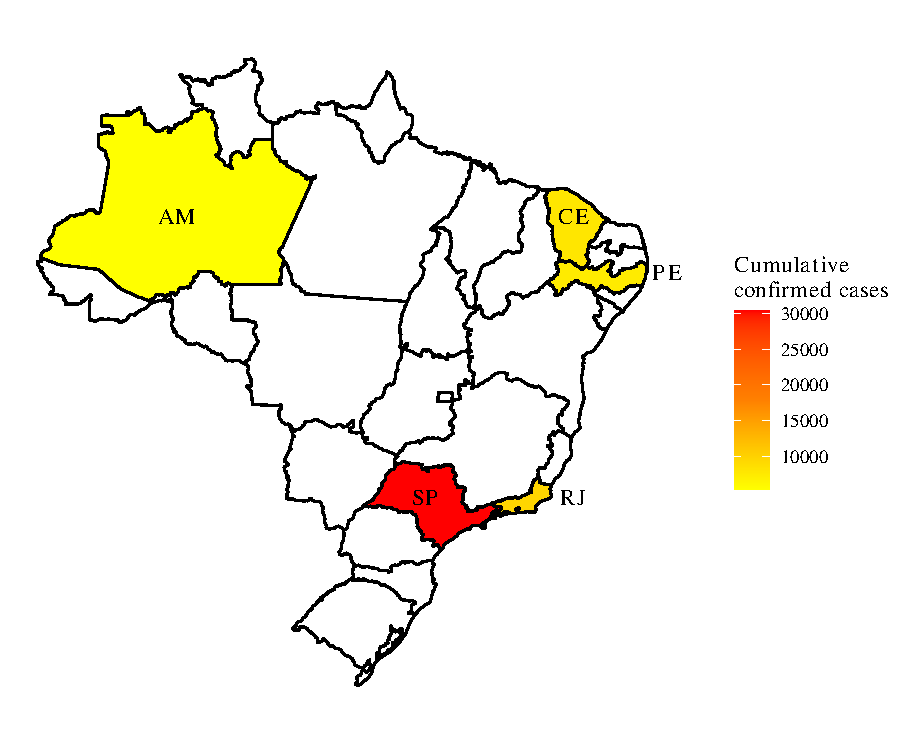
\includegraphics[width=.385\linewidth]{Media/cs1_heatmap_bra.pdf}
    % }
    % %
    % \subfloat[\ac{USA} \label{subfig:heatmap_USA}]{
    %     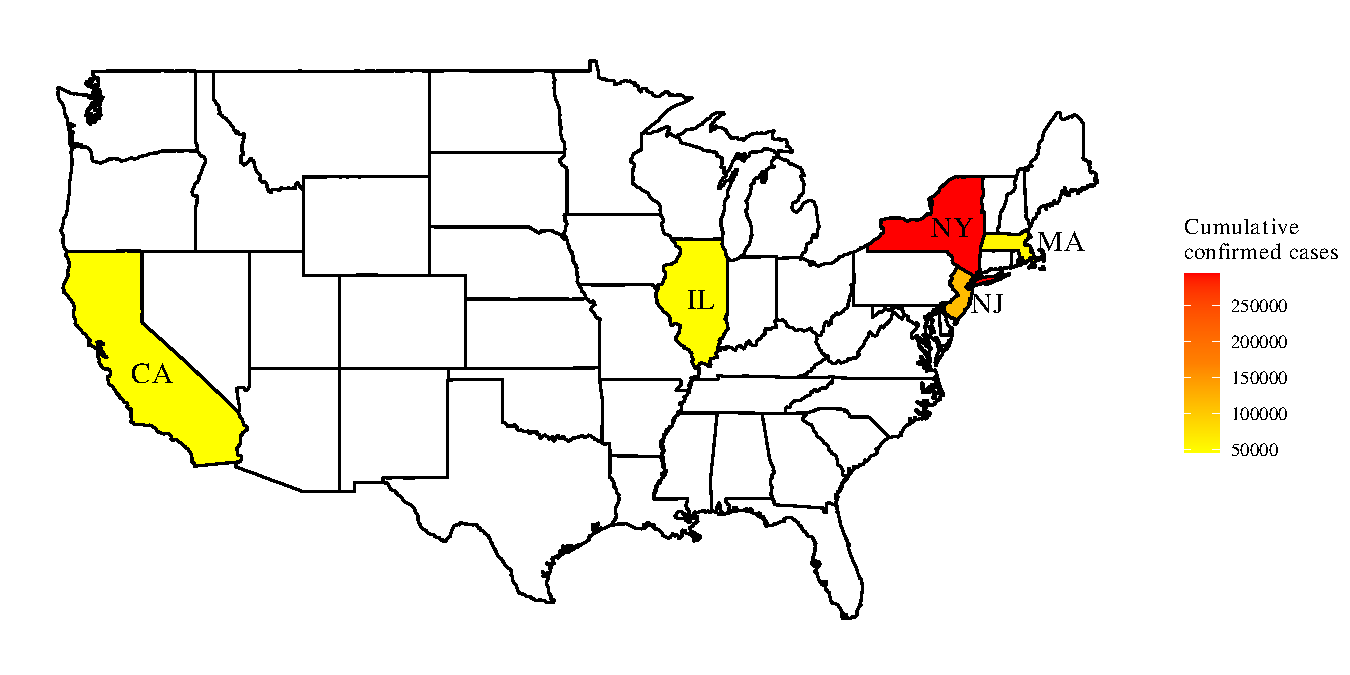
\includegraphics[width=.575\linewidth]{Media/cs1_heatmap_usa.pdf}
    % }
    \subfloat[Brazil \label{subfig:heatmap_BRA}]{
        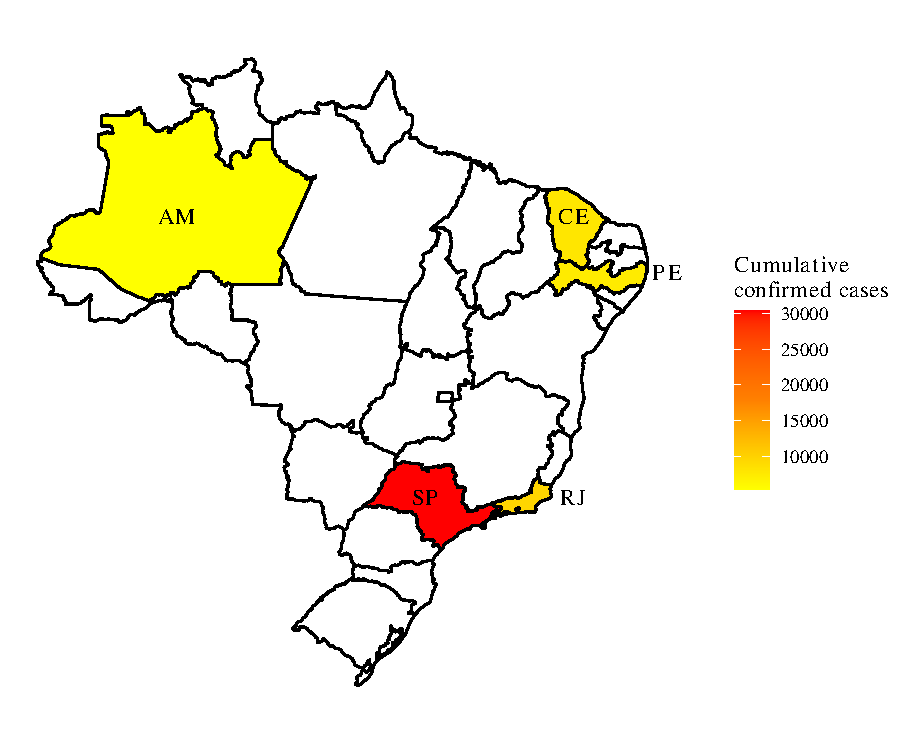
\includegraphics[width=.7\linewidth]{Media/cs1_heatmap_bra.pdf}
    }
    
    \subfloat[\ac{USA} \label{subfig:heatmap_USA}]{
        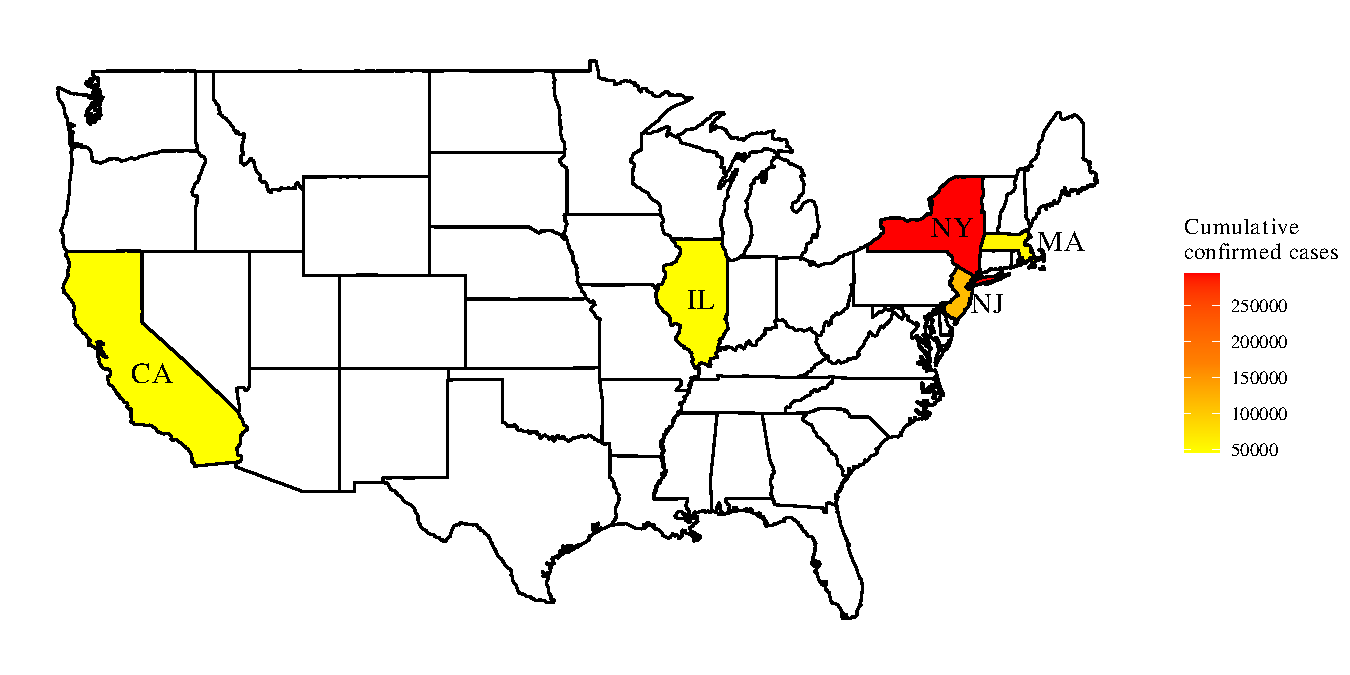
\includegraphics[width=.9\linewidth]{Media/cs1_heatmap_usa.pdf}
    }
    \caption{Heatmap of the cumulative confirmed cases to five states from Brazil and USA.}
    \label{fig:heatmap}
    \source{\citeonline{dasilva2020Forecasting}}
\end{figure}

%%%%%%%%%%%%%%%%%%%%%%%%%%%%%%%%%%%%%%%%%%%%%%%%%%

\subsection{Proposed Forecasting Framework}

This section describes the main steps in the data analysis adopted by \ac{BRNN}, \ac{CUBIST}, \ac{KNN}, \ac{QRF}, \ac{SVR}, and \ac{VMD} based models. 

\begin{enumerate}[start=1,label={\textbf{Step \arabic*:}},wide = 0pt, leftmargin = 3em]
\item \label{step1} First, the dataset output variables are decomposed into five \ac{IMF}s by performing \ac{VMD}. The lag equal 2 was chosen by grid-search, applied on the \ac{IMF}s creating four inputs from the lags, and applied on the exogenous inputs. Further, the new data is split into training and test sets. The test set consists of the last six observations, and the remaining samples define the training set. In the training state, leave one-out-cross-validation with time slice was adopted, such as developed by \citeonline{ribeiro2020Ensemble}.

\item \label{step2} Each \ac{IMF} is trained with each model presented before using the time-slice validation approach. Next, a simple summation-grouping model reconstructed the \ac{IMF} predictions. In other words, the \ac{IMF} is trained by the same model and is summed. Then, five predictions outputs were generated named \ac{VMD}--\ac{BRNN}, \ac{VMD}--\ac{CUBIST}, \ac{VMD}--\ac{KNN}, \ac{VMD}--\ac{QRF}, and \ac{VMD}--\ac{SVR}.

\item \label{step3} A recursive strategy is employed to develop multi-days-ahead \ac{COVID-19} cases forecasting \cite{ribeiro2020Shortterm}. Regarding this, one model is fitted for one-day-ahead forecasting. Then the recursive strategy uses this forecasting result as an input for the same model to forecast the next step, continuing until the desirable forecasting horizon. In this study, the aim is to obtain the cases up to $H$ next days, especially up to \ac{ODA}, \ac{TDA}, and \ac{SDA}, respectively. The following structures are considered as

\begin{equation}
    \hat{y}_{(t+h)} =
    \begin{cases}
    \hat{f}\left\{y_{(t+h-1)}, \,y_{(t+h-2)},\,\mathbf{X}_{(t+h-1)}\right\} & \text{if } h = 1, \\
    \hat{f}\left\{\hat{y}_{(t+h-1)},\,\hat{y}_{(t+h-2)},\, \mathbf{X}_{(t+h-3)}\right\} & \text{if } h = 3, \\
    \hat{f}\left\{\hat{y}_{(t+h-1)},\, \hat{y}_{(t+h-2)},\, \mathbf{X}_{(t+h-6)}\right\} & \text{if } h = 6, \\
    \end{cases}
\end{equation}
where $\hat{f}$ is a function that maps the cumulative \ac{COVID-19} cases, $\hat{y}(t+h)$ is the forecast of cumulative cases in horizon $h=$1, 3 and 6, $y(t+h-1)$, ${y}(t+h-2)$ are the previous observed, $\hat{y}(t+h-1)$, $\hat{y}(t+h-2)$ are the predicted cumulative cases, $\mathbf{X}(t+h-n_x)$ is the exogenous inputs vector at the maximum lag of inputs ($n_x = 1$ if $h = 1$, $n_x = 3$ if $h = 3$, and $n_x = 6$ if $h = 6$). All hyperparameters employed in this study are presented in Tables \ref{tab:hyper1} and \ref{tab:hyper2} in Appendix~\ref{app:cs1_appendixA}.  

\item To evaluate the effectiveness of adopted models, from obtained forecasts out-of-sample (test set), \ac{IP}, \ac{sMAPE}, and \ac{RRMSE} criteria are computed. Figure \ref{fig:flowchart} presents the proposed forecasting framework.

% FIGURE - Diagram
\begin{figure}[htb!]
    \centering
    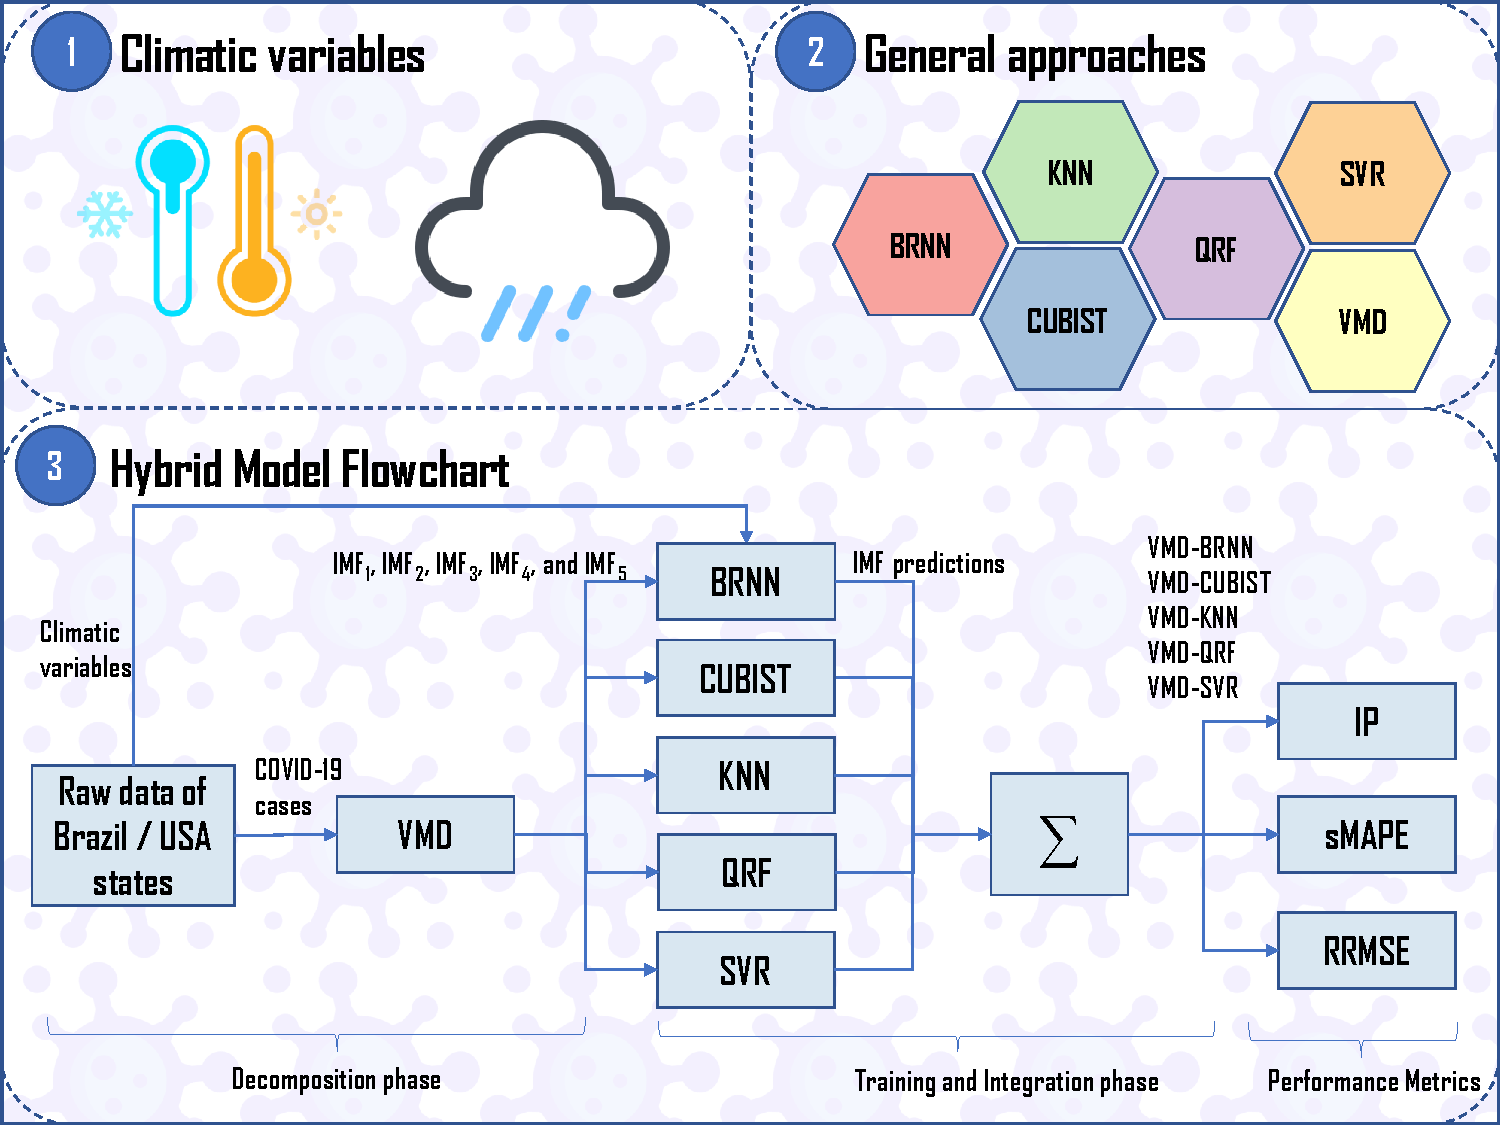
\includegraphics[width=0.9\linewidth]{Media/cs1_framework.pdf}
    \caption{Proposed forecasting framework for Application 1}
    \label{fig:flowchart}
    \source{\citeonline{dasilva2020Forecasting}}
\end{figure}

\end{enumerate}

\newpage
\section{Renewable Energy 1 Time Series} \label{sec:renewable1}

This subsection presents a contextualization, contributions, datasets, and methodology adopted for application 2.

\subsection{Contextualization and Contributions}

Renewable energy, such as wind energy, has been increasing its operation in the energy matrix in the last decades in many countries worldwide. Global Wind Energy Council expects that over 355$GW$ of new capacity will be added between 2020 - 2024, which is nearly 71$GW$ of new installations each year until 2024 \cite{globalwindenergycouncilgwec2020Market}. Even in Brazil, whose electrical power system is majority composed of hydroelectric systems (60.6\%), wind energy already has a parcel of the National energy matrix, equaling approximately 9.1\% of Brazil's source installed capacity \cite{moreno2020Multistep}, and it is the principal renewable energy sources. According to the 2020 ``Infowind'' of the \citeonline{brazilianwindenergyassociationabeeolica2020INFOWIND}, Brazil's wind power generation had 15.6$GW$ of installed capacity with 624 wind farms in March 2020, which led Brazil to be ranked as the 7th country in wind energy installed capacity. In 2019, 55.9$TWh$ of wind energy was generated, recording a growth of 15.5\% concerning the previous year. This generation supplies 88.5 million inhabitants and represents 17\% of the power the National Interconnected System consumes.

The main concern about increasing wind power generation into electrical power systems is related to maintaining the electrical system's reliability since the wind energy production can swing from 20\% up to 100\% of the wind farm capacity \cite{vatanpour2018Impact}. In an electric power subsystem with a large amount of wind power, even if this subsystem is tied-to-the-grid, the inherent and significant wind uncertainty can potentially cause severe difficulties in power system operation \cite{li2019Smart}. Especially in Brazil's Northeast region, which concentrated the largest wind farms, with higher installed capacity factor, and also considering the size and characteristics of Brazil's electrical power system, the biggest concern for the \ac{ONS} still is getting accurate wind speed forecasting to planning the daily dispatch of electrical energy, avoiding or minimizing impacts into system stability and frequency control, also reducing the excess of wind energy curtailment \cite{moreno2020Multistep}.

The issues related to wind energy growth in Brazil's Northeast region can result in 7\% of curtailments at the end of 2020 \cite{jong2017Forecasting} since the number of wind farms has been increasing and the transmission lines have already reached the maximum capacity. On the other hand, the economical solution relies on more accurate wind energy forecasting to better plan for the short term. This leads to optimal storage decisions since the region has the largest hydropower plants, and the hydropower plants have no constraints about unit commitment or load ramps \cite{jong2017Forecasting}.

Wind speed is characterized by its high level of uncertainty and nonlinear behavior. Due to these behaviors, coupled with the lack of forecasting mathematical tools to provide coherent predictions, wind energy is classified as an intermittent source, i.e., the supply of wind energy is unstable. This erratic behavior makes accurately predicting wind energy a challenge. Wind energy forecasting models can be classified by their prediction time horizon into four categories, very short, short, medium, and long-term, as illustrated in Figure~\ref{fig:leadtime} \cite{moreno2019Very}.  

\begin{figure}[!htb]
    \centering
    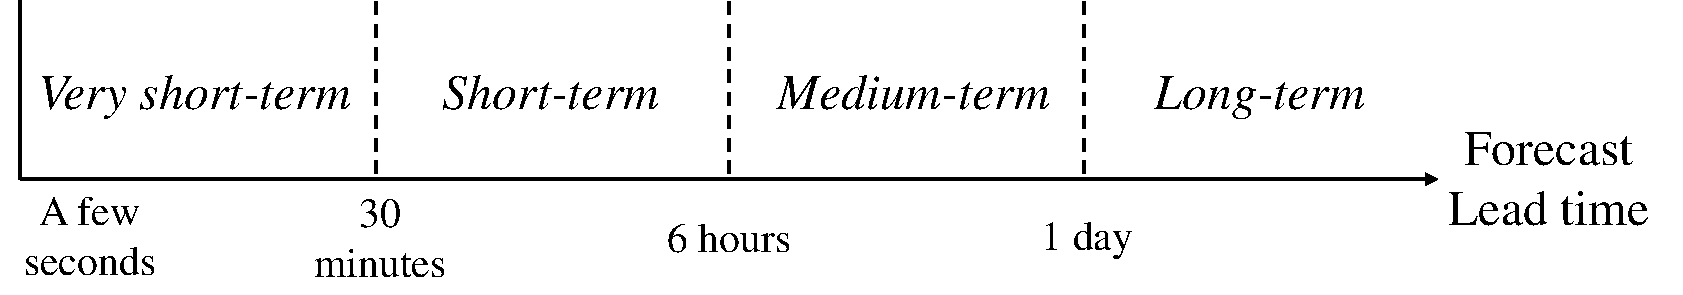
\includegraphics[width=0.9\linewidth]{Media/cs2_leadtime.pdf}
    \caption{Time-scale classification of wind energy forecasting}
    \source{\citeonline{liu2019Data}}
    \label{fig:leadtime}
\end{figure}

Usually, a shorter forecasting time horizon can provide more detailed and accurate results but less time left for the deployment of wind power generation. In comparison, a longer forecasting time horizon provides long-term information about future wind energy, but usually, the accuracy is relatively poor. At the same time, shorter forecasting time horizons, like very short and short-term, provide accurate results, and their applications are beneficial for turbine regulation and preload sharing \cite{liu2019Data}.

Despite the increasing wind power production and wind farm installed capacity in Brazil, the energy market and operation rules given by \ac{ONS} still do not represent wind energy accurately. Due to these factors, this significantly impacts investors and power system operations, primarily due to lots of wind farm curtailments imposed by load flow constrain-off \cite{ribeiro2019Desafio}. Therefore, a very short-term time horizon approach is chosen in this study, aiming to produce accurate information about wind energy production in the next 30 minutes.

The objective of this study is to develop a hybrid decomposition-ensemble learning model by using \ac{CEEMD} coupled with \ac{STACK} approach and machine learning models, such as \ac{CUBIST}, \ac{KNN}, \ac{PLS}, \ac{RIDGE}, and \ac{SVR}. In consideration of the previous objective detailed, the following \ac{RQ}s are defined:

\begin{enumerate}[wide=0pt, leftmargin=3em]
    \item[\textbf{RQ 1.2}] Can signal decomposition approaches enhance the performance of forecasting wind energy generation time series?

    \item[\textbf{RQ 3.1}] What is the improvement achieved by employing the \ac{STACK} approach coupled with signal decomposition approaches over non-decomposed models when forecasting wind energy generation time series?

    \item[\textbf{RQ 4}] Can preprocessing methods applied to the time series improve the forecasting performance of the decomposition-ensemble learning strategy?
\end{enumerate}

To address the \ac{RQ}s of this application, the contributions can be summarized as follows: 

\begin{enumerate}[label = \alph*)]
    \item The first contribution is related to evaluating the use of decomposition-ensemble learning methods for multi-step-ahead very short-term forecasting. 
    
    \item As the second contribution, we can highlight using exogenous input signals with past (delayed) wind power observations (input lags) to provide additional information to the model. 
    
    \item Third contribution lies in applying different preprocess techniques to compose the proposed hybrid forecasting method. 
    
    \item Last, this study evaluates the proposed framework forecasting in a multi-step-ahead forecasting strategy. 
\end{enumerate}

\subsection{Dataset Description}

The three collected datasets refer to the wind turbine power generation sampled on 10 minutes basis. All variables were related to a wind turbine in a wind farm in Parazinho city, Brazil. The measurement period comprises August, September, and October 2017 for each dataset, respectively, illustrated in Figure~\ref{fig:datasetscs1}. There are two main reasons for choosing data from different months: (i) more data allows models to learn as many data characteristics; and (ii) each month has its climate characteristics, allowing us to evaluate the model in different climate scenarios. Furthermore, once the data came from a private company the datasets are limited to these periods. The typical wind energy forecasting approach considers only wind speed as the input to predict the next power production on the desired number of steps ahead. However, the actual wind turbine generator operation condition introduces some effects on the next power production stage, and it can be represented in the forecasting modeling as exogenous variables. To map this effect on power forecasting, we also have considered the set of variables related to this condition as input. This set was composed by seven features such as absolute wind direction, ambient temperature, temperatures of two generators bearings, generator speed, nacelle direction, and wind speed. Last, wind power was chosen as target variable.

% Datasets
\begin{figure}[htb!]
    \centering
    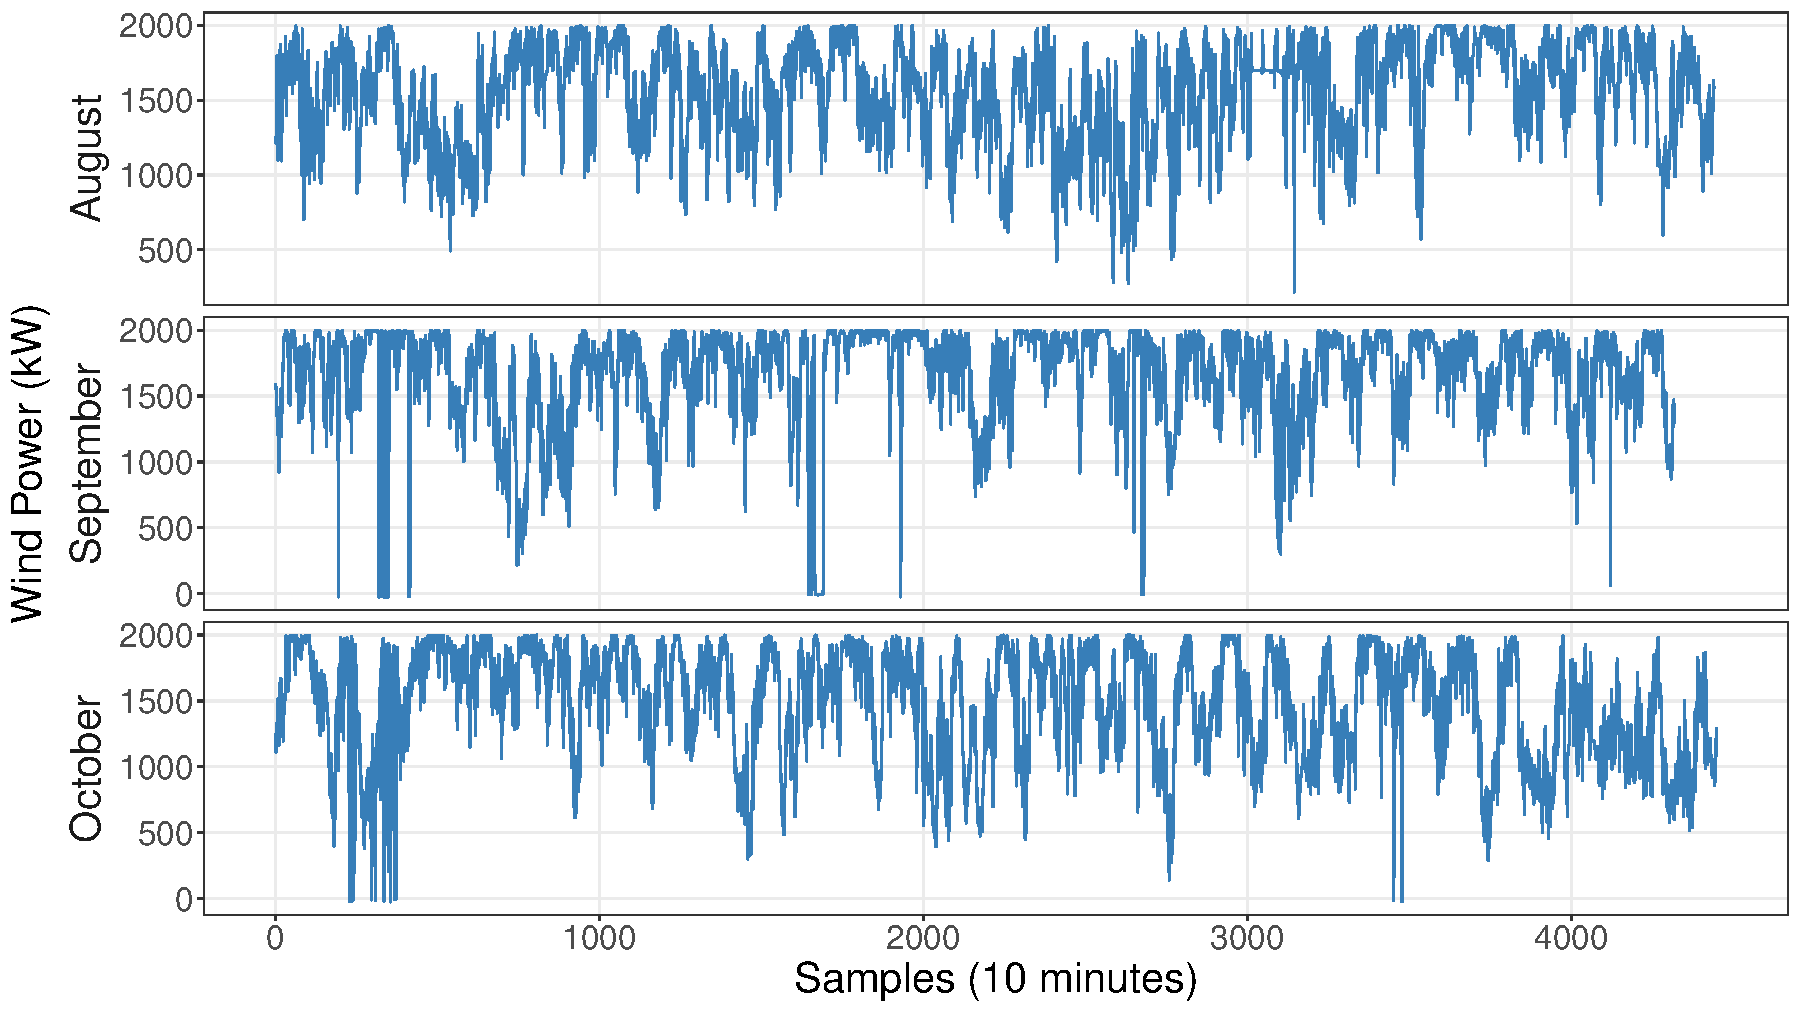
\includegraphics[width=\linewidth]{Media/cs2_datasets_plot.pdf}
    \caption{Datasets for August, September, and October 2017}
    \source{\citeonline{dasilva2021Novel}}
    \label{fig:datasetscs1}
\end{figure}

Further, the experiment split each dataset into training and test sets in the proportion of three weeks and one week, respectively. So, the test set (out-of-sample), comprising the last seven days of the month, have around 1,008 observations for each month. These proportions allow the models to learn the data pattern and behavior by using an adequate number of observations and make it possible to evaluate the learning in a sufficient number of values. Also, other proportions used in the literature were analysed such as 80 and 20\%, 75 and 25\%, and 70 and 30\%, however the proportion of three weeks for training set and one week for test was chosen due to interpretability and usability of the model by the company that provided the data. Table~\ref{tab:summary} presents an overview of the statistical indicators of the three datasets, which are mean, standard deviation (Std), minimum (Min), and maximum (Max).

\begin{landscape}
\begin{scriptsize}
\begin{center}
\begin{longtable}[htb!]{llllll|llll|llll}
\caption{Summary of the statistical indicators of the inputs and output of the datasets \label{tab:summary}} \\
\hline
\multirow{3}{*}{\textbf{Variable (Unit Measure)}} & \multirow{3}{*}{\textbf{Samples}} & \multicolumn{12}{c}{\textbf{Statistical indicator}} \\ \cline{3-14}
 & & \multicolumn{4}{c|}{August} & \multicolumn{4}{c|}{September} & \multicolumn{4}{c}{October} \\ \cline{3-14}
 & & Mean & Std & Min & Max & Mean & Std & Min & Max & Mean & Std & Min & Max \\ \hline \endfirsthead
  \multicolumn{14}{c}{\tablename\ \thetable\ -- \textit{Continued from previous page}} \\ \hline

\multirow{3}{*}{\textbf{Variable (Unit Measure)}} & \multirow{3}{*}{\textbf{Samples}} & \multicolumn{12}{c}{\textbf{Statistical indicator}} \\ \cline{3-14}
 & & \multicolumn{4}{c|}{August} & \multicolumn{4}{c|}{September} & \multicolumn{4}{c}{October} \\ \cline{3-14}
 & & Mean & Std & Min & Max & Mean & Std & Min & Max & Mean & Std & Min & Max \\ \hline \endhead \hline \multicolumn{14}{r}{\textit{Continued on next page}} \\
\endfoot
\hline
\endlastfoot

                                         
Power ($kW$)                             & Whole                    & 1553.02 & 338.82 & 217.5  & 2000.3 & 1652.78 & 395.46 & -24.7 & 2000.3 & 1478.57 & 422.85 & -25.3 & 2000.1 \\
                                         & Training                 & 1511.48 & 341.27 & 217.5  & 2000.3 & 1638.16 & 423.06 & -24.7 & 2000.3 & 1529.83 & 411.88 & -25.3 & 2000.1 \\
                                         & Test                     & 1694.46 & 288.64 & 572.4  & 2000.1 & 1700.81 & 281.57 & 61.4  & 2000.1 & 1303.64 & 413.11 & -24.8 & 1997.5 \\ \hline
Absolute Wind                            & Whole                    & 134.24  & 13.2   & 97.6   & 167.2  & 153.95  & 17.95  & 106.4 & 193.3  & 128.91  & 13.26  & 83.4  & 162.3  \\
Direction (Degrees)                      & Training                 & 134.31  & 13.28  & 97.6   & 167.2  & 159.46  & 15.81  & 106.4 & 193.3  & 130.36  & 12.01  & 93.9  & 160.9  \\
                                         & Test                     & 133.98  & 12.91  & 103.8  & 162.9  & 135.87  & 11.54  & 107.7 & 159.9  & 123.94  & 15.86  & 83.4  & 162.3  \\ \hline
Ambient Temperature                      & Whole                    & 26.04   & 2.49   & 22     & 32     & 25.75   & 2.61   & 22    & 32     & 26.51   & 2.63   & 23    & 33     \\
(Celsius)                                & Training                 & 25.94   & 2.44   & 22     & 31     & 25.66   & 2.57   & 22    & 32     & 26.37   & 2.66   & 23    & 33     \\
                                         & Test                     & 26.39   & 2.61   & 23     & 32     & 26.05   & 2.7    & 22    & 31     & 26.96   & 2.48   & 24    & 32     \\ \hline
Generator Bearing                        & Whole                    & 63.46   & 6.6    & 46     & 76     & 66.62   & 7.35   & 44    & 80     & 63.18   & 8.79   & 44    & 81     \\
Temperature (Celsius)                    & Training                 & 62.45   & 6.5    & 46     & 76     & 66.46   & 7.54   & 44    & 80     & 64.03   & 8.61   & 44    & 81     \\
                                         & Test                     & 66.89   & 5.69   & 50     & 75     & 67.17   & 6.65   & 50    & 78     & 60.27   & 8.77   & 46    & 79     \\ \hline
Generator Bearing 2                      & Whole                    & 49.98   & 4.59   & 39     & 59     & 51.44   & 4.9    & 39    & 60     & 50.03   & 5.64   & 38    & 64     \\
Temperature (Celsius)                    & Training                 & 49.38   & 4.55   & 39     & 59     & 51.3    & 4.96   & 39    & 60     & 50.55   & 5.6    & 38    & 64     \\
                                         & Test                     & 52.02   & 4.13   & 41     & 58     & 51.92   & 4.64   & 42    & 60     & 48.25   & 5.44   & 39    & 60     \\ \hline
Generator Speed (RPM)                    & Whole                    & 1282.16 & 75.08  & 335    & 1345.4 & 1293.32 & 169.49 & 0     & 1345.8 & 1253.17 & 121.96 & 0     & 1345.6 \\
                                         & Training                 & 1276.64 & 78.36  & 335    & 1345.4 & 1290.69 & 190.22 & 0     & 1345.8 & 1261.69 & 123.14 & 0     & 1345.6 \\
                                         & Test                     & 1300.94 & 58.87  & 1009.5 & 1345   & 1301.95 & 64.51  & 184.4 & 1345.1 & 1224.1  & 113.18 & 53.2  & 1344.9 \\ \hline
Nacelle Direction                        & Whole                    & 134.13  & 13.28  & 98.7   & 165.6  & 153.76  & 18.46  & 4.9   & 254.2  & 128.87  & 13.33  & 83.5  & 164    \\
(Degrees)                                & Training                 & 134.23  & 13.43  & 98.7   & 165.6  & 159.21  & 16.61  & 4.9   & 254.2  & 130.34  & 12.09  & 91.6  & 164    \\
                                         & Test                     & 133.78  & 12.74  & 104.2  & 161.9  & 135.87  & 11.69  & 109.4 & 162.1  & 123.88  & 15.91  & 83.5  & 160.4  \\ \hline
Wind Speed ($m/s$)                       & Whole                    & 9.24    & 1.18   & 5.1    & 15.4   & 10.5    & 1.67   & 5.2   & 17.2   & 9.02    & 1.32   & 4.7   & 13.8   \\
                                         & Training                 & 9.15    & 1.2    & 5.1    & 15.4   & 10.75   & 1.72   & 5.2   & 17.2   & 9.17    & 1.33   & 4.7   & 13.8   \\
                                         & Test                     & 9.52    & 1.06   & 6.3    & 12.6   & 9.69    & 1.14   & 6.5   & 13.3   & 8.52    & 1.14   & 5.4   & 12.5   \\ \hline
\end{longtable}
\end{center}
\end{scriptsize}
\end{landscape}

\subsection{Proposed Forecasting Framework}

The proposed model will be applied to train \ac{IMF}s and the residue generated by the decomposition step aiming to forecast the wind power generation in a multi-step-ahead forecasting strategy. Each dataset output was decomposed into five different \ac{IMF}s and one residue by \ac{CEEMD} (six components in total). The training process was performed by \ac{KNN}, \ac{PLS}, \ac{RIDGE}, and \ac{SVR} with the linear kernel as base-learners (weak model), and \ac{CUBIST} as meta-learner (strong model), for stack's layer-0 and layer-1, respectively, applied into each one of the six components. The component predictions in layer-0 are summed, giving four different predictions, one for each weak model. Those are applied as inputs for layer-1, where they were preprocessed using three other techniques: \ac{BC}, \ac{CORR}, and \ac{PCA}. The meta-learner training process of the three approaches was performed by \ac{CUBIST}, resulting in three proposed models, named \ac{CEEMD}--\ac{BC}--\ac{STACK}, \ac{CEEMD}--\ac{CORR}--\ac{STACK}, and \ac{CEEMD}--\ac{PCA}--\ac{STACK}, respectively. The step-by-step of the proposed methodology is given as follows:

\begin{enumerate}[start=1,label={\textbf{Step \arabic*:}},wide = 0pt, leftmargin = 3em]
\item The datasets' output variables are decomposed into five \ac{IMF}s and one residue by performing \ac{CEEMD} (six components). The datasets decomposition are illustrated in Figure~\ref{fig:IMFs}.

\begin{figure}[htb!]
    \centering
    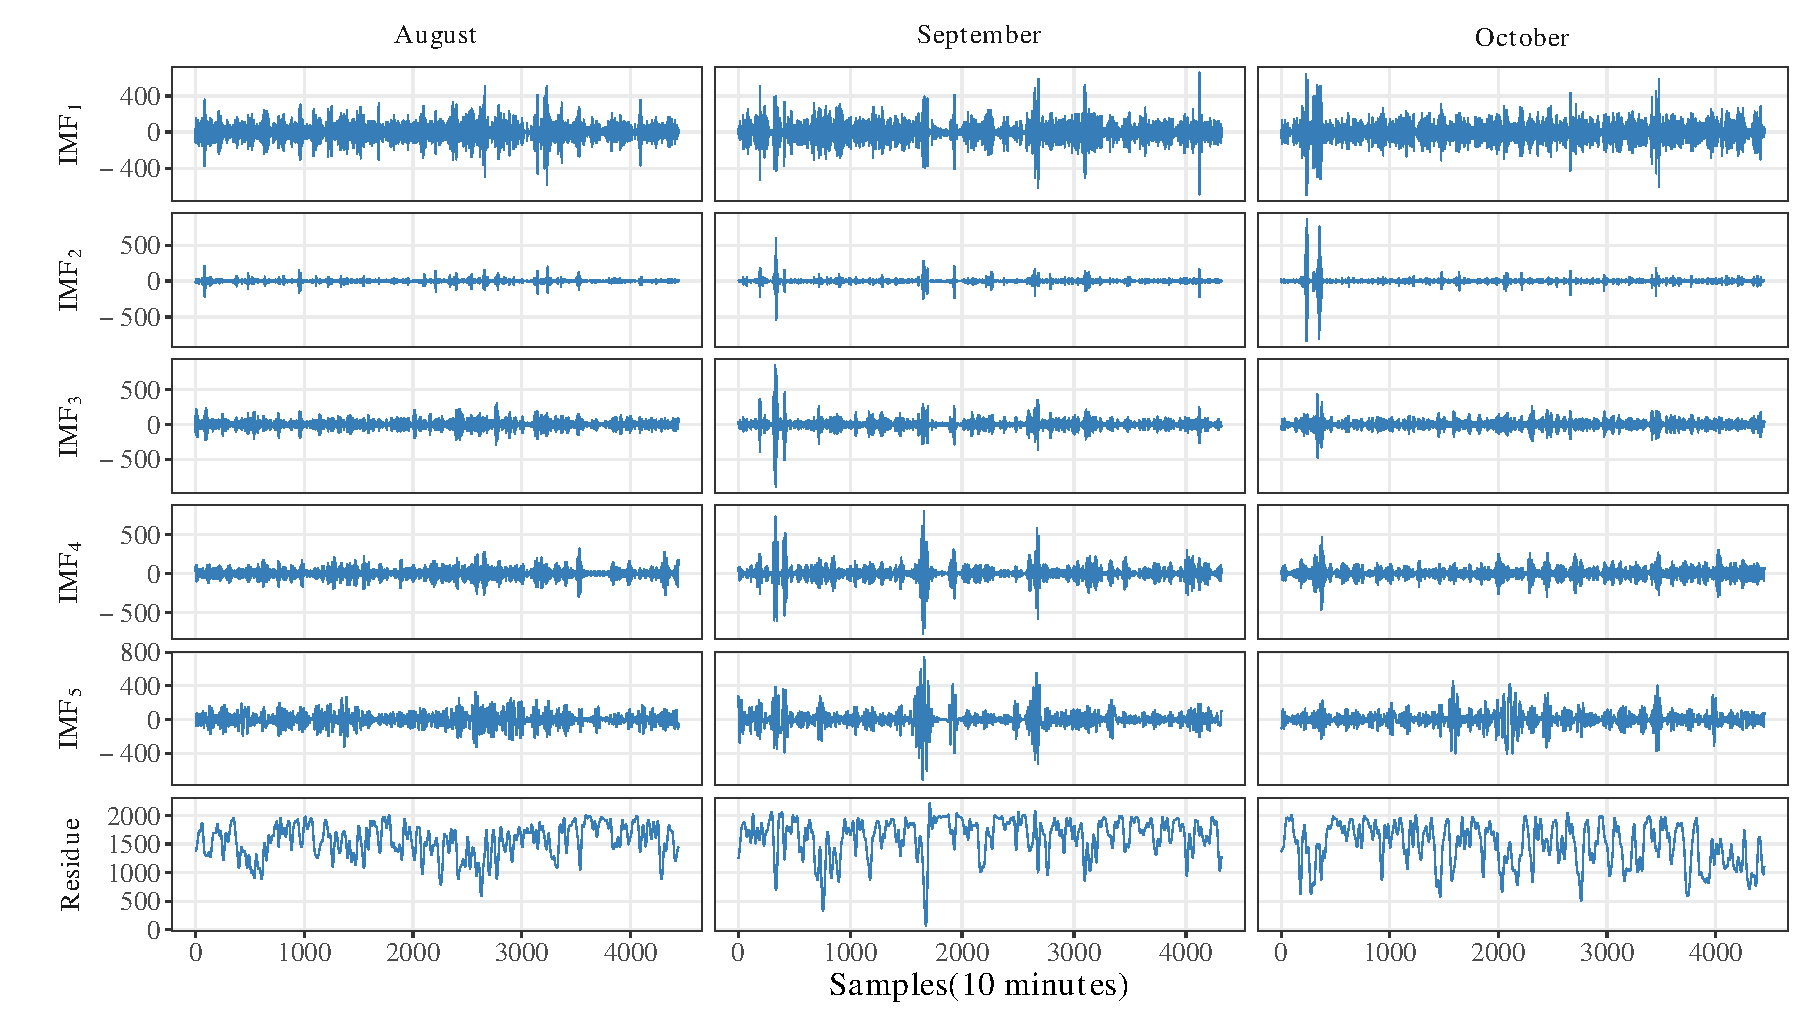
\includegraphics[width=\linewidth]{Media/cs2_imf_plot}
    \caption{Datasets decomposed into IMFs and Residue by CEEMD}
    \source{\citeonline{dasilva2021Novel}}
    \label{fig:IMFs}
\end{figure}

\item The lag equals 4 was chosen, applied on the \ac{IMF}s creating four inputs from the lags, and lay on the exogenous inputs as well.

\item A \ac{BC} preprocess was applied on the \ac{IMF}s and the inputs in layer-0 of the stacking-ensemble learning.

\item Training each decomposition component with each base-learner model aforementioned using 5-fold cross-validation with a recurssive forecasting strategy.

\item A simple summation-grouping model reconstructed the component predictions. In other words, the components trained by the same base-learner model are summed \cite{dasilva2020Forecasting}. Then, four prediction outputs were generated named \ac{CEEMD}--\ac{KNN}, \ac{CEEMD}--\ac{PLS}, \ac{CEEMD}--\ac{RIDGE}, and \ac{CEEMD}--\ac{SVR}.

\item The four prediction outputs generated in layer-0 were used as input in layer-1. They were preprocessed using \ac{BC}, \ac{CORR} which removes those predictors whose correlation was greater than a threshold, and \ac{PCA}. Then, training each model using \ac{CUBIST} as meta-learner in layer-1 of the \ac{STACK} gives three different final predictions, which are the proposed models, named \ac{CEEMD}--\ac{BC}--\ac{STACK}, \ac{CEEMD}--\ac{CORR}--\ac{STACK}, and \ac{CEEMD}--\ac{PCA}--\ac{STACK}, respectively. To forecast 10, 20, and 30-minutes-ahead the applied structures are defined, respectively, as

\begin{scriptsize}
\begin{equation}
\hat{y}(t+h) = \begin{cases}
\hat{f}\left\{y(t+h-1),y(t+h-2),y(t+h-3),y(t+h-4),\mathbf{X}(t+h-1)\right\} & \text{if } h = 1, \\
\hat{f}\left\{\hat{y}(t+h-1),y(t+h-2),y(t+h-3),y(t+h-4),\mathbf{X}(t+h-2)\right\} & \text{if } h = 2, \\
\hat{f}\left\{\hat{y}(t+h-1),\hat{y}(t+h-2),y(t+h-3),y(t+h-4),\mathbf{X}(t+h-3)\right\} & \text{if } h = 3,
\end{cases}
\end{equation}
\end{scriptsize}
where $\hat{f}$ is a function that maps the wind power generation, $\hat{y}(t+h)$ is the forecast of wind power generation in horizon $h=$1 and 3 at time $t$ ($1,\ldots, 140$), $y(t+h-1)$, ${y}(t+h-2)$, ${y}(t+h-3)$, ${y}(t+h-4)$ are the previous observed, $\hat{y}(t+h-1)$, $\hat{y}(t+h-2)$ are the predicted wind power generation, $\mathbf{X}(t+h-n_x)$ is the exogenous inputs vector at the maximum lag of inputs ($n_x = 1$ if $h = 1$, {$n_x = 2$ if $h = 2$}, and $n_x = 3$ if $h = 3$).

\item Performance metrics (\ac{MAE}, \ac{MAPE}, and \ac{RMSE}) and statistical hypothesis tests (\ac{DM} test) were conducted to evaluate the accuracy of the proposed models compared to (i) different preprocess techniques applied in the layer-1 phase; (ii) \ac{CEEMD} models without \ac{STACK} method; (iii) \ac{STACK} models without decomposition and different preprocess techniques; and (iv) the models applied directly to the dataset. 

Hence, as described in this Section, the proposed model framework is illustrated in Figure~\ref{fig:frameworkcs1}.

% FIGURE - Framework
\begin{figure}[htb!]
    \centering
    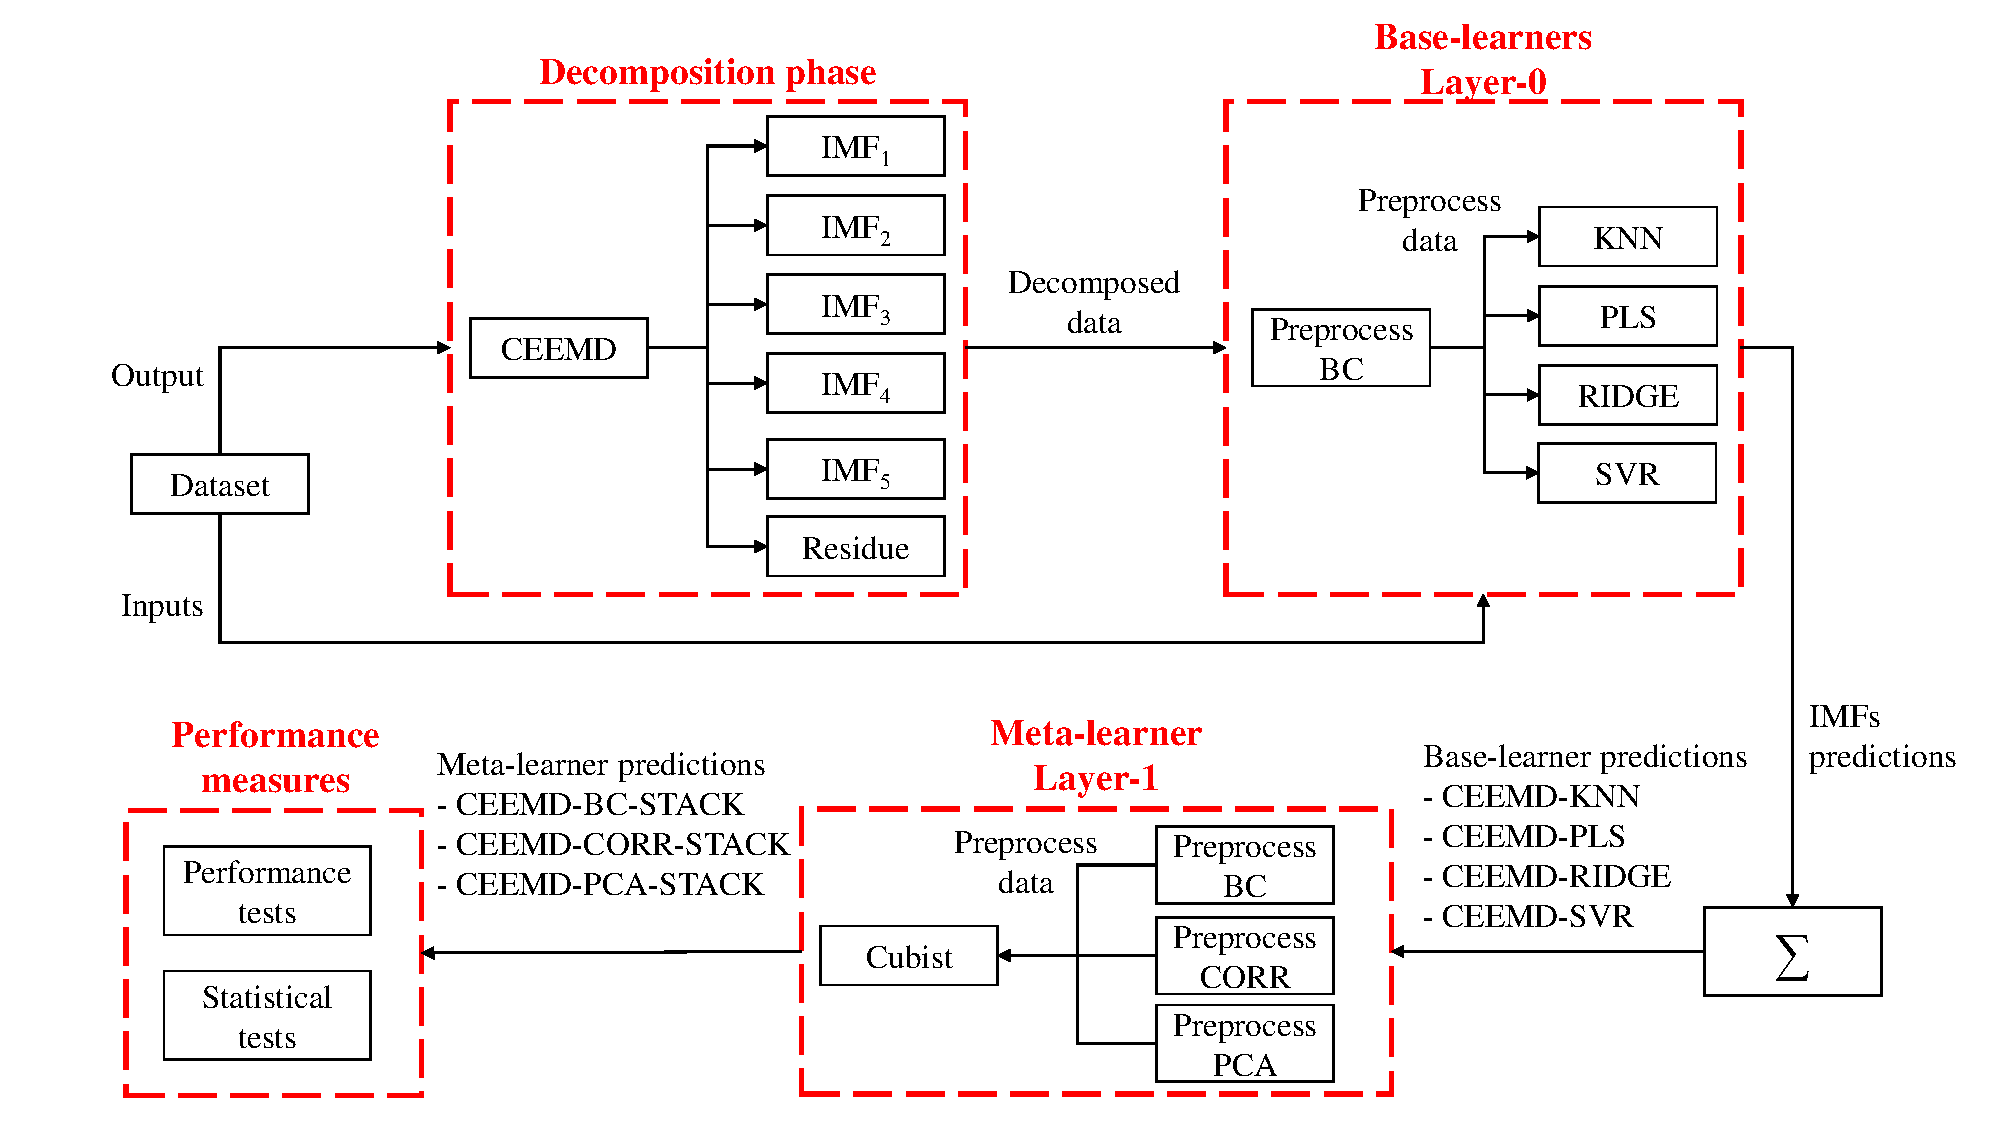
\includegraphics[width=\textwidth]{Media/cs2_framework.pdf}
    \caption{Proposed forecasting framework for Application 2 \label{fig:frameworkcs1}}
    \source{\citeonline{dasilva2021Novel}}
\end{figure}

\end{enumerate}

\newpage
\section{Renewable Energy 2 Time Series} \label{sec:renewable2}

This subsection presents a contextualization, contributions, datasets, and methodology adopted for application 3.

\subsection{Contextualization and Contributions}

Over the past few decades, wind energy in many nations worldwide has increased its role in the energy matrix. Between 2020 and 2024, the Global Wind Energy Council anticipates that more than 355 $GW$ of new capacity will be installed, including about 71 $GW$ of new plants every year up to 2024 \cite{globalwindenergycouncilgwec2020Market}. Wind power, including in Brazil, has a considerable part of the national energy grid. The electric energy system mainly comprises hydroelectric energy (57.8\% of energy output), one of the primary renewable energy sources. In line with the \citeonline{brazilianwindenergyassociationabeeolica2021Energia} study of 2021, ``Infowind'', as of February 2021, Brazil is now 7th in the world with 18 $GW$ of installed wind energy capacity from more than 8,300 wind-energy turbines, spread throughout 695 wind farm areas on the coast of Brazil. Wind energy generated 55,9 $TWh$ in 2019, an increase of 15.5\% over the previous year. This generation feeds 88.5 million people and accounts for 17\% of the total energy utilized in the interconnected national network.

Notwithstanding the wind energy expansion, the central issue is the electricity grid's reliability since wind energy generation can once swing between 20 and 100 percent of the wind farm's capability owing to intermittent wind properties \cite{vatanpour2018Impact}. In different terms, wind energy is identified as an intermittent source, making its supply unpredictable due to the high level of insecurity and the nonlinear behavior of the wind speed \cite{dasilva2021Novel}. The \ac{ONS} primary key is establishing reliable wind speed forecasts to plan daily electrical energy dispatch. That avoids or limits system stability and frequency regulation impacts and lowers wind energy curtailment surplus \cite{moreno2020Multistep}.

Therefore, an accurate wind speed forecast is crucial for asset management and the electrical system operator. Wind speed forecasting across various horizons is critical for turbine regulation, electricity market clearing, energy allocation, electric power management, and equipment maintenance schedules. Wind speed prediction models may also be categorized into four groups, very short, short, medium, and long-term, by their predicted time horizon \cite{liu2019Data}. A shorter prediction time frame may produce more comprehensive and accurate findings, but there is less time for deploying wind power generation. On the other hand, a lengthier forecasting time horizon gives long-term knowledge on future wind energy, but the accuracy is typically decreased \cite{moreno2019Very}.

Forecasting short-term wind speed as precisely as possible is essential to the energy market and \ac{ONS} due to wind characteristics and the present Brazilian electrical system condition. Therefore, this study aims to offer a hybrid forecasting system that combines \ac{SSA} and \ac{VMD} with machine learning methods and \ac{STACK}. The model will train the elements obtained in the decomposition, striving to forecast the short-term wind speed in a multi-step manner (10, 30, and 60 minutes ahead horizon). In consideration of those as mentioned above, the following \ac{RQ}s are defined:

\begin{enumerate}[wide=0pt, leftmargin=3em]
    \item[\textbf{RQ 1.3}] Can signal decomposition approaches enhance the performance of forecasting wind speed time series?

    \item[\textbf{RQ 3.2}] What is the improvement achieved by employing \ac{STACK} approach coupled with signal decomposition approaches over non-decomposed models when forecasting wind speed time series?

    \item[\textbf{RQ 5}] Can the multi-stage signal decomposition strategy outperform the single-stage signal decomposition approach?

    \item[\textbf{RQ 6}] Can the employment of \ac{STACK} method improve the forecasting performance of the multi-stage signal decomposition strategy?
\end{enumerate}

To address the \ac{RQ}s of this application, the contributions can be summarized as follows:

\begin{enumerate}[label=\alph*)]

    \item The use of multi-stage signal decomposition for short-term wind speed forecasting. Combining two decomposition techniques (\ac{SSA} and \ac{VMD}) to compose a two-stage signal decomposition technique, the \ac{VMD} performed the first stage, and \ac{SSA} performed the second stage. This process is also evaluated accordingly.
    
    \item The use of the stacked generalization ensemble learning framework coupled with multi-stage signal decomposition for short-term wind speed forecasting. The stacking-ensemble learning scheme can enhance the performance of the multi-stage signal decomposition framework by its divide-and-conquer characteristic, making the model more robust.
    
    \item Using different machine learning forecasting models combined with the multi-stage signal decomposition and stacking-ensemble learning approaches. The reason for choosing different models to compose the \ac{STACK} model is due to the diversity of the models' characteristics, in which the \ac{STACK} approach can extract the best from each model.
    
\end{enumerate}

\subsection{Dataset Description}

The dataset utilized as input in the proposed framework consists of three months of wind speed measurements. The measurements are made every 10 min at a height 95 meters from ground level, corresponding to a wind generator with a blade diameter of 100 meters. The measurement apparatus is installed to monitor the wind resource for a wind farm, with approximately 150 $MW$ capacity, located in the State of Rio Grande do Norte, in the Northeastern region of Brazil, more specifically at Parazinho city. The measurements are made from March until May 2020. The time series is created out of 4,464 samples for March and May 2020 and 4,320 samples for April 2020, with a sampling period of 10 min, as presented in Figure~\ref{fig:datasets}. Using data from different months is essential because further data permit models to learn the maximum number of data features. Also, it has its climatic characteristics each month and thus makes it possible to assess the pattern in various climate situations \cite{dasilva2021Novel}. Furthermore, once the data came from a private company the datasets are limited to these periods.

% Figure - datasets
\begin{figure}[htb!]
    \centering
    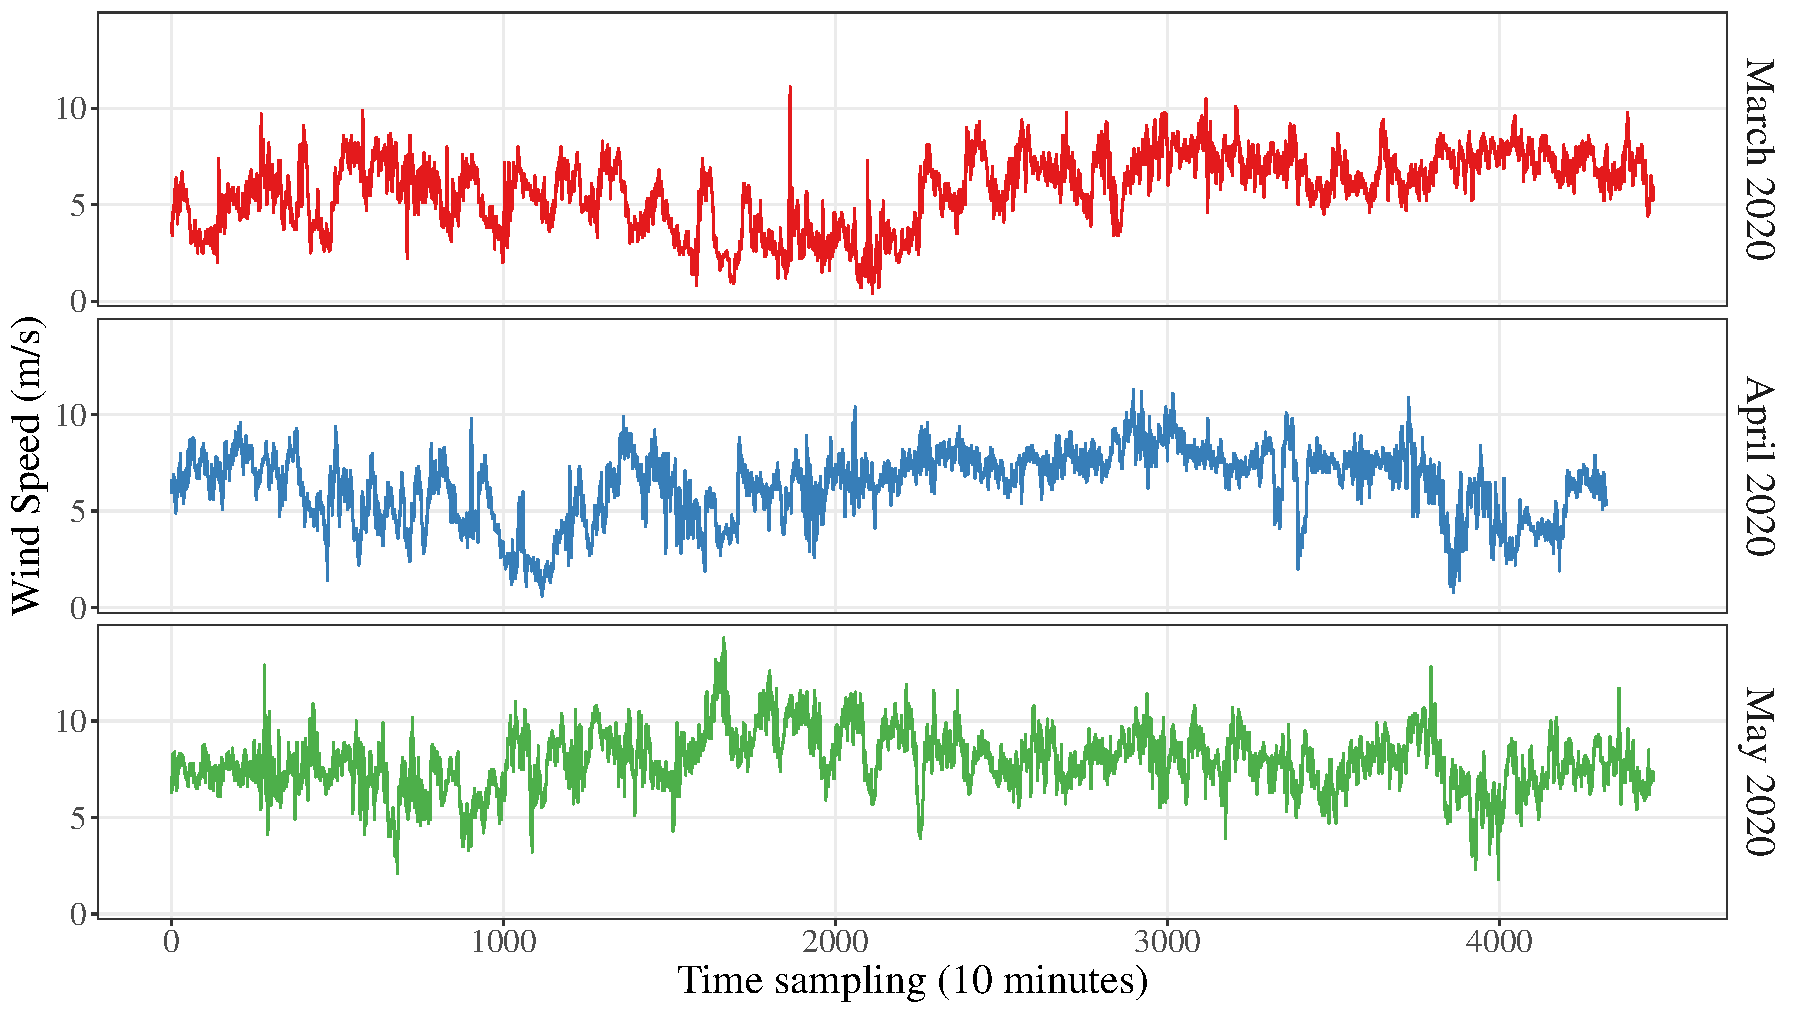
\includegraphics[width=\linewidth]{Media/cs3_datasets_plot.pdf}
    \caption{Datasets for March, April, and May 2020, respectively}
    \label{fig:datasets}
    \source{\citeonline{dasilva2022Multistep}}
\end{figure}

Moreover, the datasets were sequentially divided into training and test sets for three and one weeks. Then, the test set, corresponding to the out-of-sample data, and composed of the last seven days of the month, has about 1,008 observations each month. Those proportions were enough so that models could learn the patterns and behavior of the data, with a sufficient number of observations to give a fair number of points to evaluate the learning procedure. Also, other proportions used in the literature were analysed such as 80 and 20\%, 75 and 25\%, and 70 and 30\%, however the proportion of three weeks for training set and one week for test was chosen due to interpretability and usability of the model by the company that provided the data.

\subsection{Proposed Forecasting Framework}

The proposed model is made out of two decomposition stages. First, the decomposition using \ac{VMD}, and, subsequently, the decomposition using \ac{SSA}. \ac{VMD} extracts the trend components from each original dataset output. The remaining signal is decomposed into four other parts using \ac{SSA}, so each time series is decomposed into five components by \ac{VMD} and \ac{SSA}.

The \ac{RIDGE}, \ac{KNN}, \ac{SVR} with linear kernel, and \ac{PLS} are evaluated as the layer-0 base learners in the training process. In layer-1, the \ac{CUBIST} model is trained. The predictions of each component of layer-0 are added (for every individual model) to form each model's forecast. The predictions of the base learners are used as input for the layer-1 meta-learner. The predictions of the meta-learner form this study's proposed model named \ac{VMD}--\ac{SSA}--\ac{STACK}. The models' performances are evaluated by using \ac{IP}, \ac{MAE}, \ac{MAPE}, \ac{RMSE}, \ac{RRMSE}, and \ac{SSE} performance metrics. Furthermore, the \ac{DM} hypothesis test is employed to evaluate the statistical significance of the difference in errors of the models. The framework for the proposed model is illustrated in Figure~\ref{fig:framework} and explained in further detail in the following steps.

% Figure - Framework
\begin{figure}[htb!]
    \centering
    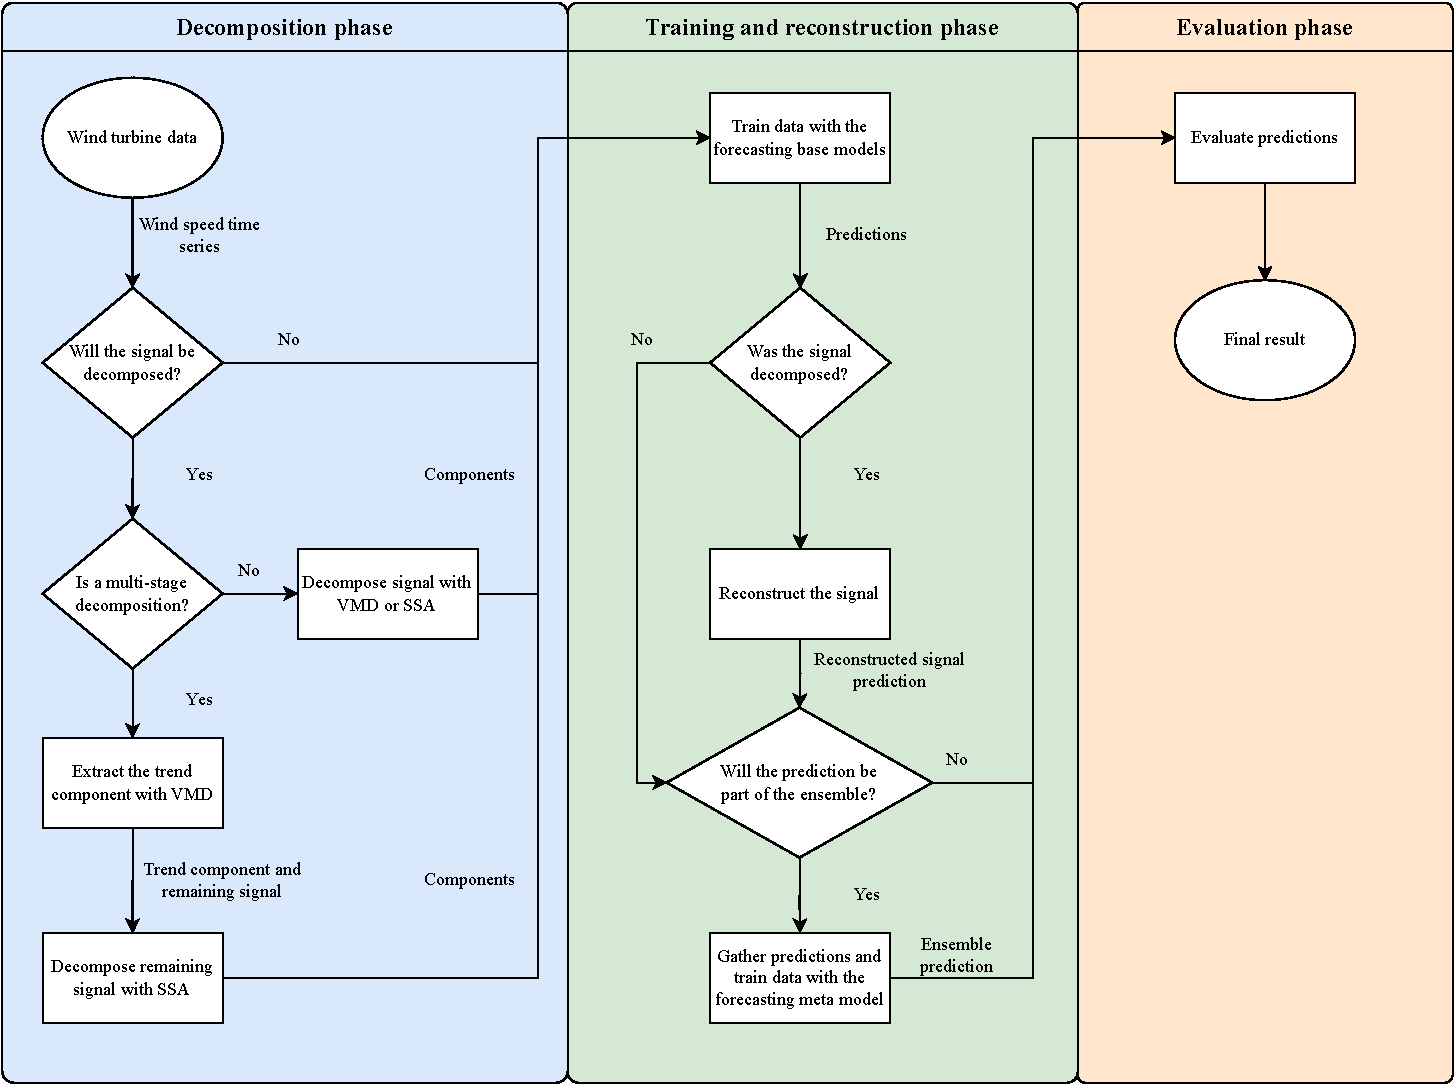
\includegraphics[width=\textwidth]{Media/cs3_framework.pdf}
    \caption{Proposed forecasting framework for Application 3}
    \label{fig:framework}
    \source{\citeonline{dasilva2022Multistep}}
\end{figure}

\begin{enumerate}[start=1,label={\textbf{Step \arabic*:}},wide = 0pt, leftmargin = 3em]
\item First, the \ac{VMD} was performed to extract the trend component ($c_1$) from the original time series. The difference between the original time series and $c_1$ was calculated, resulting in a high-frequency signal. \ac{SSA} decomposed this remaining signal into four other components ($c_2$ up to $c_5$). The main idea of the hybrid multi-stage decomposition is to use \ac{VMD} as the first decomposition method due to its characteristic of dealing with high oscillatory signals by suppressing the high-frequency noise from the components generated. Therefore, \ac{VMD} extracts the band-limited trend component from the signal, while the \ac{SSA} decomposes the remaining signal into a trend, seasonal, oscillations, and aperiodic noises. The five components are presented in Figure~\ref{fig:comps}.

% Figure - components
\begin{figure}[htb!]
    \centering
    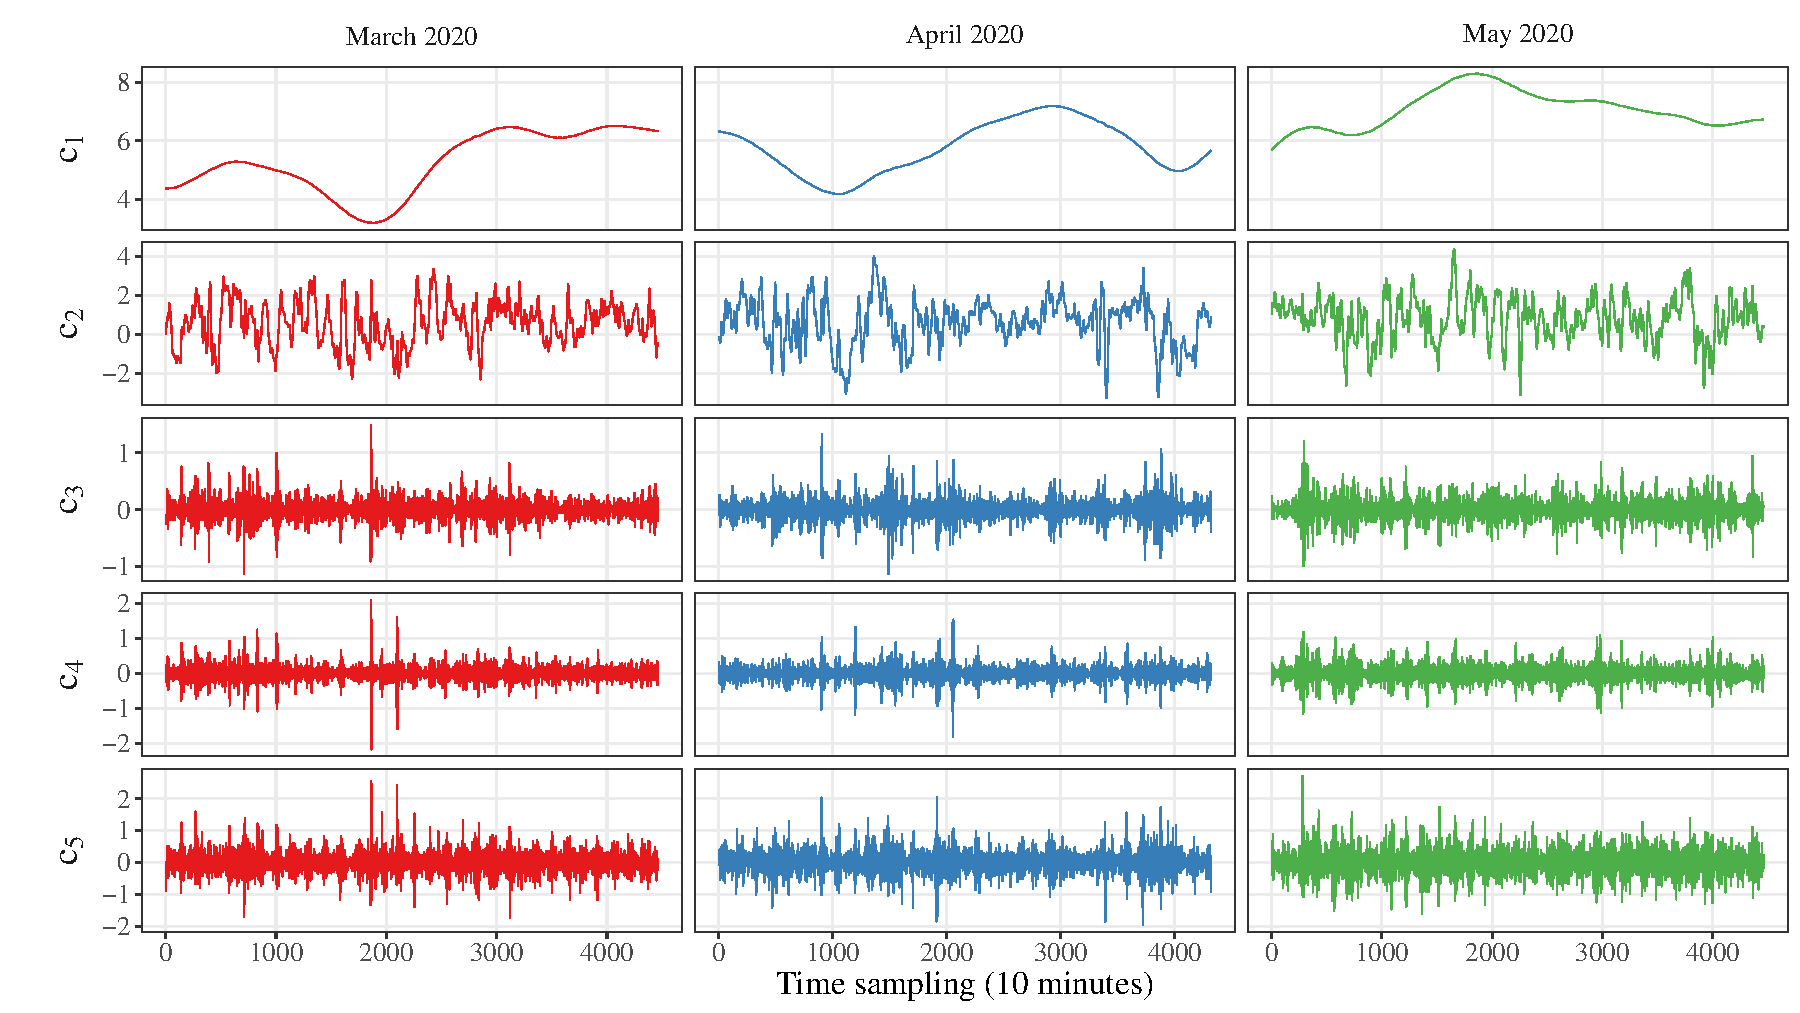
\includegraphics[width=\linewidth]{Media/cs3_imf_plot.pdf}
    \caption{Datasets decomposed into components by VMD and SSA approaches}
    \label{fig:comps}
    \source{\citeonline{dasilva2022Multistep}}
\end{figure}

The value of 5 lags was determined via grid-search and used to transform the data into a format suited to supervised learning models. The data is then split into train and test sets. The test data is made from the last 1,008 measurements, which are the previous seven days of the dataset, while the training is performed with the remaining samples. The train and test sets are in the proportion of 77.5\% and 22.5\%, respectively, sufficient for the models to learn data patterns in the problem in this study. Parameters for \ac{VMD} and \ac{SSA} decomposition are shown in Table \ref{tab:settings} on Appendix~\ref{app:hyper3}. For \ac{SSA}, $C$ is the number of components of the \ac{SSA} procedure, and $n$ is the length of the time series. Regarding \ac{VMD}, $\alpha$ is the balancing parameter of the data fidelity constraint, $\tau$ is the time-step of the dual ascent (usually we can pick 0 for noise-slack), $k$ the number of modes to be recovered from \ac{VMD}, and the iteration number which is triggered if do not converge at tolerance level.

In a scheme in which each component is predicted individually, like the one used in this study and shown in Figure \ref{fig:framework}, the relationship between the number of components and the number of parameters needs to be addressed as more models result in more parameters \cite{moreno2020Multistep}. It is possible to analyze the contribution of every eigenvalue $\lambda_i$ from the singular value decomposition to determine the number of resulting components from the decomposition procedures, which is related to how much each one contributes to the complete time series. This contribution can be estimated by
%
\begin{equation}
    \textit{\%Contribution} = \frac{\lambda_i}{\sum_{i=1}^{l}\lambda_i}.
    \label{eq:eigen}
\end{equation}

% Figure - spectrum
\begin{figure}[htb!]
    \centering
    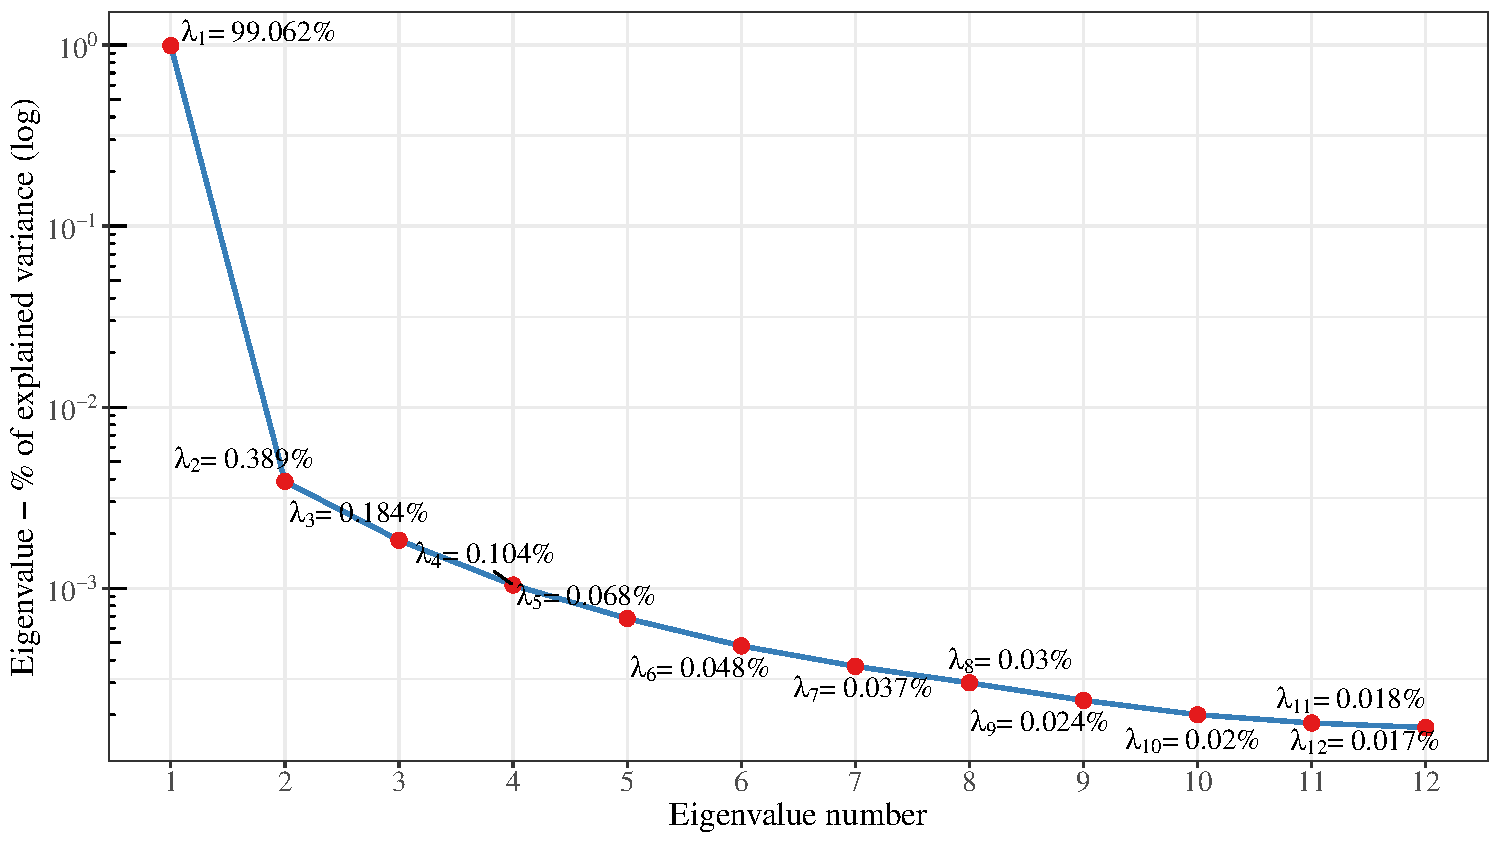
\includegraphics[width=.9\linewidth]{Media/cs3_spectrum.pdf}
    \caption{Explained variance by each eigenvalue number}
    \label{fig:spectrum}
    \source{\citeonline{dasilva2022Multistep}}
\end{figure}

Figure \ref{fig:spectrum} shows the contribution of every eigenvalue for the time series of March 2020. The contribution is considerably small after the second eigenvalue ($\lambda_2$). After the fifth eigenvalue, the sum of contributions is equal to 0.194\%. According to \citeonline{moreno2020Multistep}, this is an important metric to make a better decision considering the trade-off where increasing the number of components it will increase the number of parameters related to forecasting model that needed to be adjusted. Hence, using this analysis helps determine how much adding new parameters to the model by adding new components could help to improve the results further. As shown in Figure \ref{fig:spectrum}, the number of five components was chosen since, according to this analysis, it could explain 99.81\% of the variance of the time series.

\item For every component, the models aforementioned were trained using a 5-fold cross-validation, as in \citeonline{ribeiro2022Efficient} and \citeonline{dasilva2021Novel}, forming the base-models of the \ac{STACK}. Subsequently, the component predictions for every model are summed up by the model, creating forecasts for the single models with decomposition. With this, the four single models with decomposition predictions are generated: \ac{VMD}--\ac{SSA}--\ac{KNN}, \ac{VMD}--\ac{SSA}--\ac{PLS}, \ac{VMD}--\ac{SSA}--\ac{RIDGE}, and \ac{VMD}--\ac{SSA}--\ac{SVR}.

\item The prediction outputs from base-learners (layer-0) are used as input for the \ac{STACK}'s top layer (layer-1) meta-learner training. The meta-learner was built using a \ac{CUBIST} model. These predictions are then the predictions of the proposed model, named \ac{VMD}--\ac{SSA}--\ac{STACK}. Moreover, Table \ref{tab:hyperparameters} on Appendix~\ref{app:hyper3} shows the proposed model's hyperparameters for this study. These are the hyperparameters for every model, dataset, and forecasting horizon. The hyperparameters were defined using a grid-search for the base learners and the meta-learner.

\item A recursive strategy is utilized for multi-step ahead forecasts of this work \cite{dasilva2021Novel}. For this method, the model is fitted to a one-step-ahead forecast. The output of the first step is used as input for the second step. This process is repeated as often as needed to achieve the desired horizon. The forecast value in $t+1$ is always used to obtain the forecast in $t+2$ and subsequently for the next steps, with $t$ as the present time. This scheme is represented in Figure \ref{fig:recursive}, where the blue color represents the known actual values, the green color represents the values from the forecast of previous steps, and the yellow color represents the value being predicted in the given stage. Using this configuration, for a six-steps ahead forecast and five lagged values as input, none of the inputs are actual observed values by the sixth step ($t+6$), and only forecast values of previous steps are considered.

% Figure - recursive framework
\begin{figure}[htb!]
    \centering
    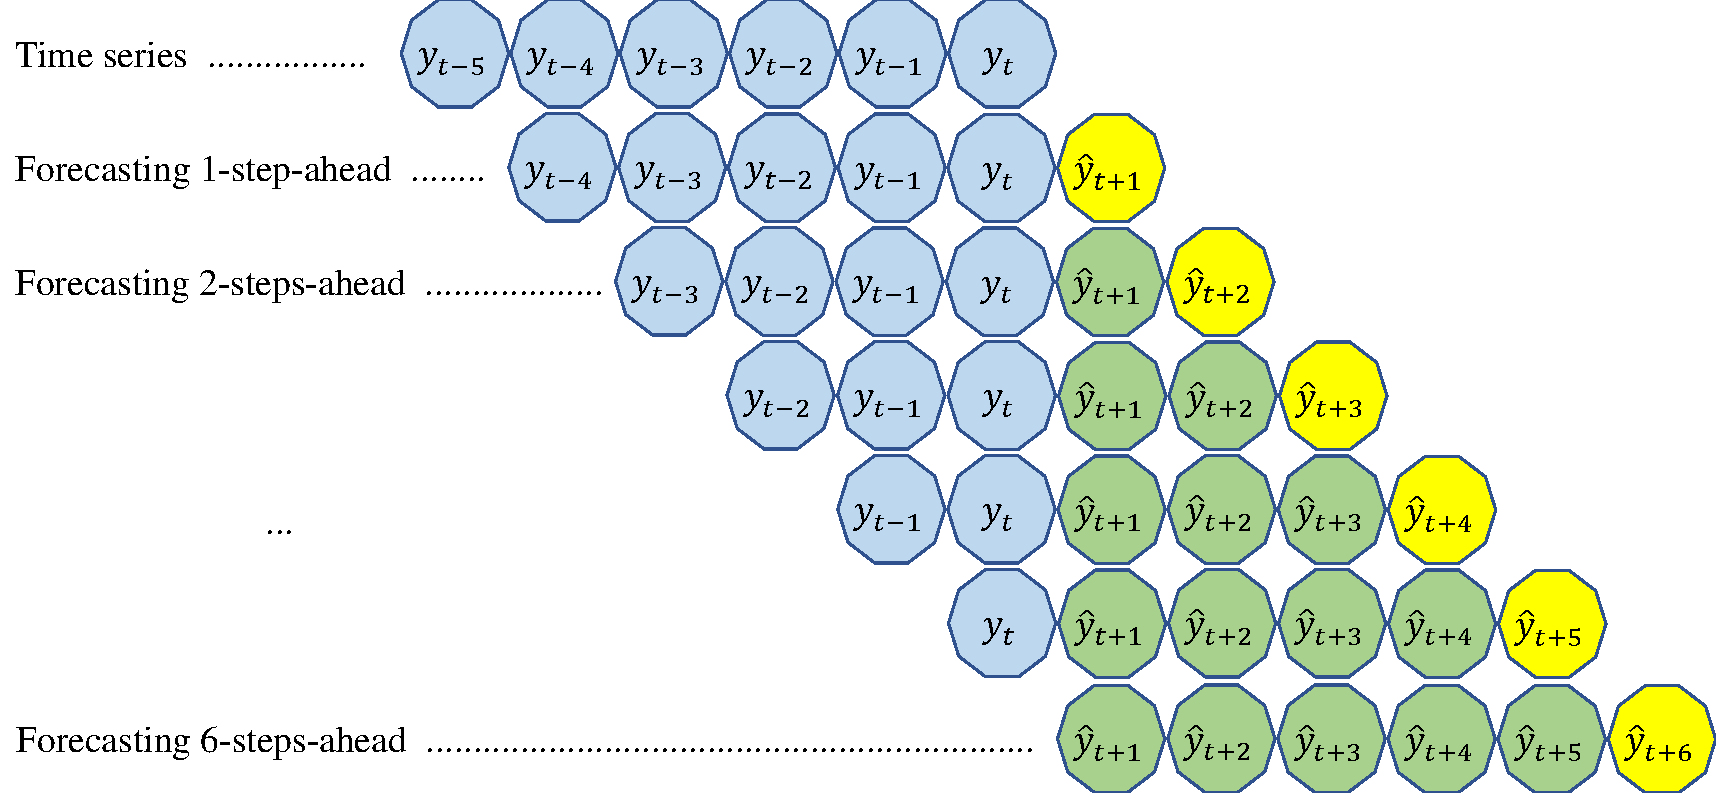
\includegraphics[width=0.85\textwidth]{Media/cs3_recursive-diagram.pdf}
    \caption{Recursive strategy of forecasting exemplified for 6-steps ahead}
    \label{fig:recursive}
    \source{\citeonline{dasilva2022Multistep}}
\end{figure}

In this study, forecasts for the $H$ next step are possible for the proposed model. For the analysis, forecasts for one, three, and six steps are produced. The following equation represents the structure for each horizon,

\begin{equation}
    \hat{y}_{(t+h)} =
    \begin{cases}
    % \left\{\begin{array}{ll}
    \hat{f}\left\{{y}_{(t+h-1)},\,{y}_{(t+h-2)},\,{y}_{(t+h-3)},\,{y}_{(t+h-4)},\,{y}_{(t+h-5)}\right\} & \textnormal{if } h = 1, \\
    \hat{f}\left\{\hat{y}_{(t+h-1)},\,\hat{y}_{(t+h-2)},\,{y}_{(t+h-3)},\,{y}_{(t+h-4)},\,{y}_{(t+h-5)}\right\} & \textnormal{if } h = 3, \\
    \hat{f}\left\{\hat{y}_{(t+h-1)},\,\hat{y}_{(t+h-2)},\,\hat{y}_{(t+h-3)},\,\hat{y}_{(t+h-4)},\,\hat{y}_{(t+h-5)}\right\} & \textnormal{if } h = 6, \\
    % \end{array}
    % \right.
    \end{cases}
\end{equation}
where $\hat{f}$ is a function that maps the wind speed, $\hat{y}_{(t+h)}$ is the forecast of wind speed in time $t$ in horizon $h=$1, 3, and 6, $y_{(t+h-1)}$ up to $y_{(t+h-5)}$ are the previous observed, $\hat{y}_{(t+h-1)}$ up to $\hat{y}_{(t+h-5)}$ are the predicted wind speed.

\item To evaluate the effectiveness of adopted models, the \ac{IP}, \ac{MAE}, \ac{MAPE}, \ac{RMSE}, \ac{RRMSE}, and \ac{SSE} performance criteria are performed. Furthermore, a \ac{DM} test is conducted to evaluate whether or not the forecasts have statistically significant differences in the residue to significance levels of 1\% and 5\%.

\end{enumerate}

